%===================================================================================================
%===================================================================================================
\chapter{計測実験と評価}
%---------------------------------------------------------------------------------------------------
\section{概要}
本研究の位置同定実験には大きく屋内実験と屋外実験に分けられる.\par
まず,屋内実験では壁に人為的にテクスチャ画像を張らない通常の屋内環境でステレオカメラを用いて実験し,位置同定精度を評価する.次に,屋内は屋外に比べるとステレオカメラが認識できる特徴が少ないため,特徴を人為的な作ったテクスチャーを壁などに貼ったまま実験を行い,位置同定精度評価する.屋内実験により最も位置同定の効率かつ精度良いパラメータ設定を求める.パラメータの種類としてはボクセルの大きさと地図・計測データのオーバーラップ有無がある.最後に,屋内実験ではKinect V2との精度比較をするため,ステレオカメラの位置同定が効率・精度良く収束できるパラメータに設定した状態で,テクスチャーを貼ったまま,Kinect V2との比較実験を行い,位置同定精度評価する.\par
屋外実験では,まず,ステレオカメラとKinect V2の日光の影響によるデータ比較実験を行い,評価する.その次に,屋内で求めた効率・精度良いパラメータに設定した状態で,屋外実験を行い,位置同定精度を評価する.最後に,屋外の一本の木の特徴を用いるだけで,位置同定が可能かについて実験を行い,評価する.一本木の実験でも屋内で求めたパラメータ設定で実験を行う.

\newpage

本研究の位置同定実験は全て,パラメータ条件を以下のようにして行う.

\begin{itemize}
\item ボクセルサイズ
\begin{itemize}
\item 80,40cm(オーバーラップ有とオーバーラップ無)
\end{itemize}
 \item パーティクル数
\begin{itemize}
      \item 初回:1000個*72方向 = 72000個
	\item 2回以降:1000個
\end{itemize}
 \item リサンプリング後の予測範囲
\begin{itemize}
      \item sigma-pos = 20[mm]
      \item 位置:現在のパーティクル かつ sigma-pos*ガウス分布
	\item sigma-ori = 2[rad]
      \item 方向:現在のパーティクル かつ sigma-ori*ガウス分布 
\end{itemize}
\item リサンプリング回数 = 100回
\item 1条件当たり5回の試行
\item オーバーラップNDボクセル
\begin{itemize}
      \item オーバーラップNDボクセルを利用(オーバーラップ有と表記)
	\item オーバーラップNDボクセルを利用しない(オーバーラップ無と表記)
\end{itemize}
\item 人為的に作成したテクスチャ
\begin{itemize}
      \item テクスチャを利用(テクスチャ有と表記)
	\item テクスチャを利用しない(テクスチャ無と表記)
\end{itemize}
\end{itemize}

\newpage

\section{屋内実験}

\subsection{テクスチャー無の屋内位置同定実験・評価}
まず,テクスチャー無の屋内実験の様子を図4.1に表す.

%
\vspace{5mm}
\begin{figure}[htbp]
  \begin{center}
   \includegraphics[height=120mm]{figure/テクスチャー無の屋内実験のキャップチャ-.eps}
   \caption{テクスチャー無の屋内実験の様子}
   \label{テクスチャー無の屋内実験のキャップチャ-}
  \end{center}
\end{figure}

\newpage

テクスチャー無の屋内位置同定実験場所をPTX形式にし,MeshLabで見たデータを図{\ref{屋内実験場所}}に表す.\par
%
\begin{figure}[htbp]
  \begin{center}
   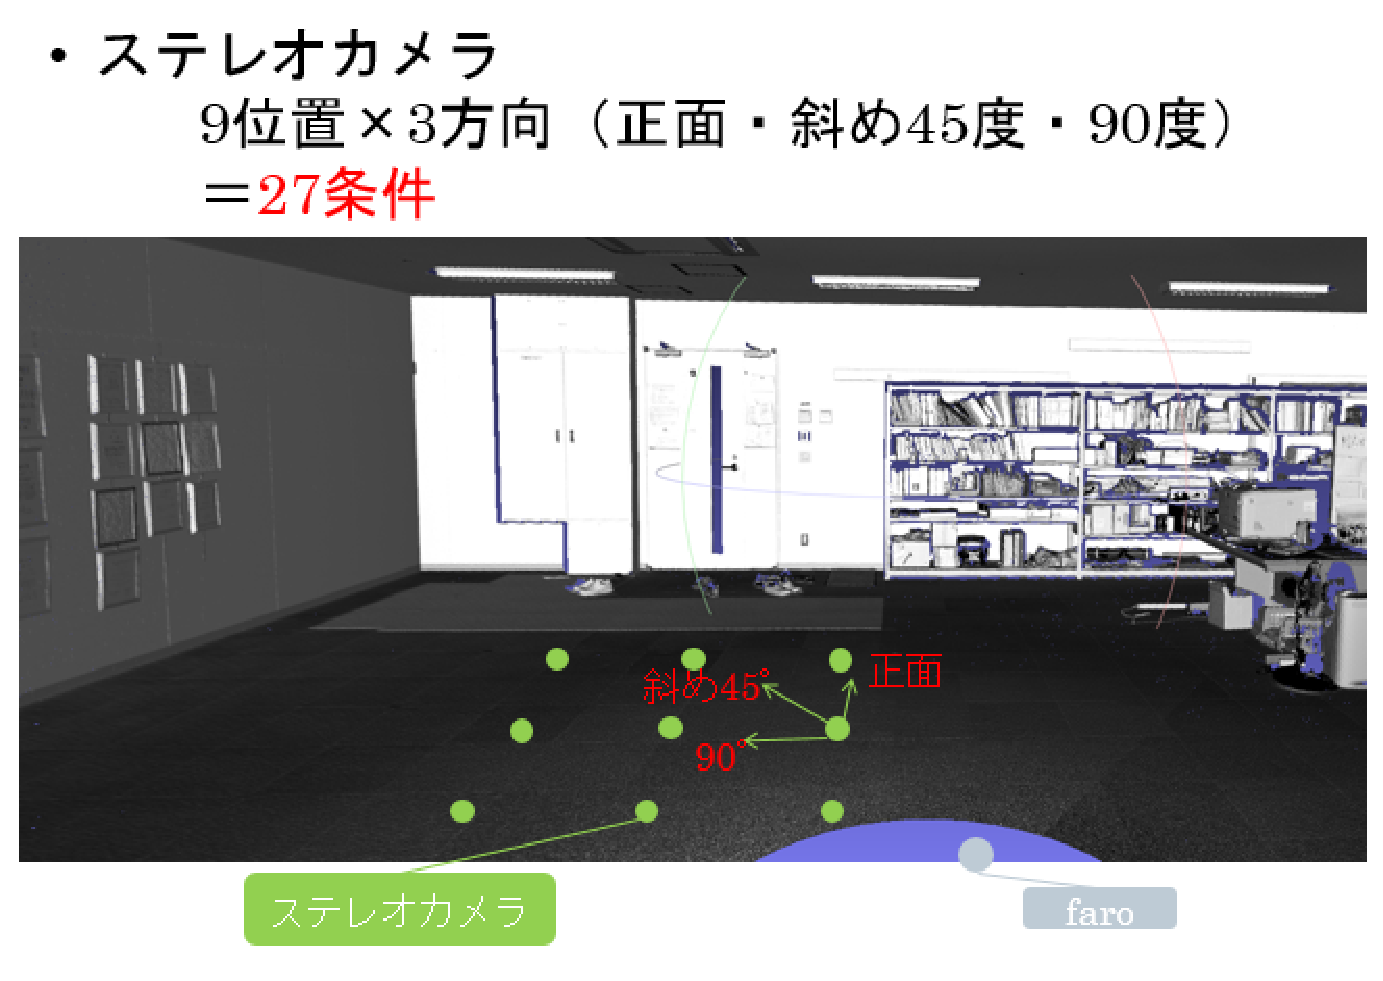
\includegraphics[height=100mm]{figure/屋内実験場所.eps}
   \caption{テクスチャー無の屋内実験場所}
   \label{屋内実験場所}
  \end{center}
\end{figure}
%

図{\ref{屋内実験場所}}のようにFAROを置いた場所は灰色の点で,ステレオカメラを用いて計測した場所は緑点の9位置である.ステレオカメラの計測は9位置から3方向(正面・斜め45度・90度),全27条件で行う.正面向きの壁からの距離は3,4,5mである.各距離で計測した計測データの例をRGB画像,PTXデータとして図{\ref{屋内計測データ例}}に表す.

\newpage
%
\begin{figure}[htbp]
  \begin{center}
   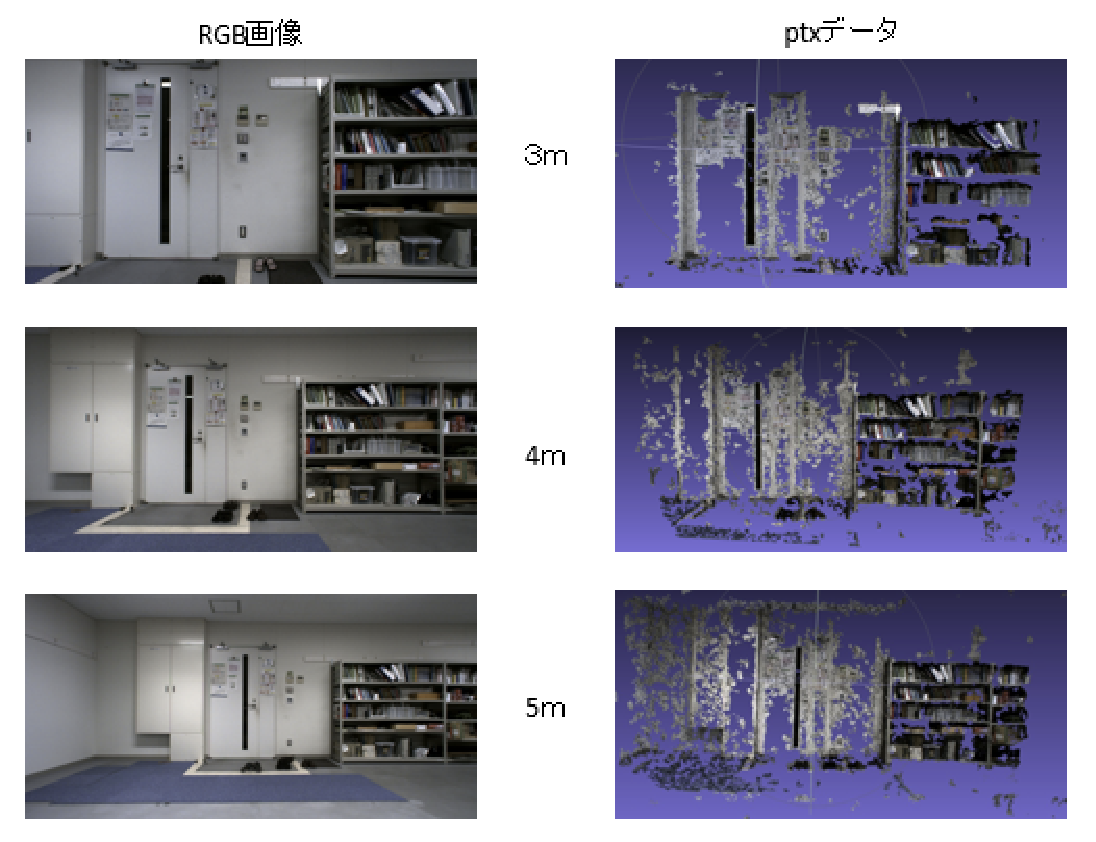
\includegraphics[height=120mm]{figure/屋内計測データ例.eps}
   \caption{テクスチャー無の屋内計測データ例}
   \label{屋内計測データ例}
  \end{center}
\end{figure}
%

位置同定プログラム上でパーティクルフィルタを使うときは乱数を与えているため,毎回同じ位置に収束するとは限らない.屋内実験の場合,地図データと計測データの収束性能を確かめるために,同じデータを用いて5回ずつ繰り返して位置同定を行い,台車の真位置から50cm以内で方向が10°以内の誤差であれば位置同定成功とみなす.本実験のパラメータの調整対象はボクセルサイズ80,40cmと地図・計測データのオーバーラップ有無となる.テクスチャー無の屋内位置同定結果をパラメータ毎に図4.4~図4.7で表す.図中の\%は試行5回中の成功率であり,右下の数字は平均の成功率(収束性能)である.



%
\begin{figure}[htbp]
  \begin{center}
   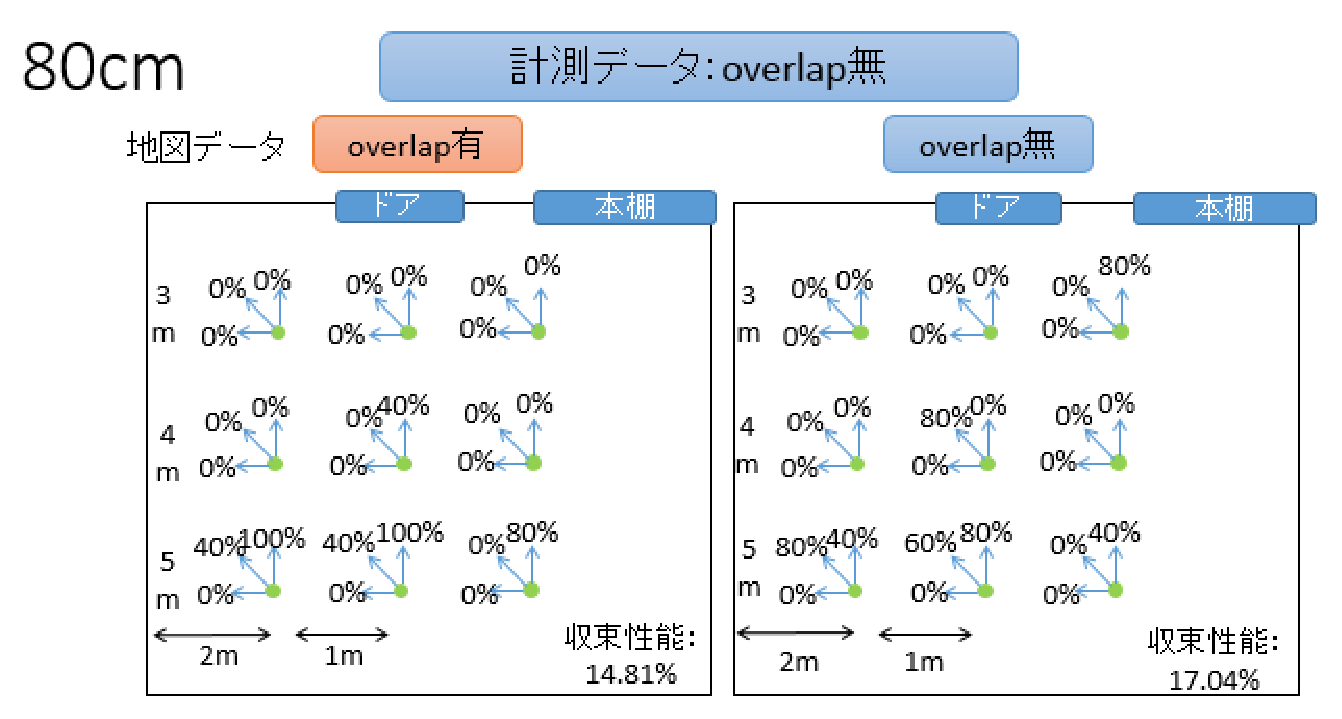
\includegraphics[height=80mm]{figure/無有無.eps}
   \caption{ボクセルサイズ:80cm,計測データオーバーラップ無かつ地図データオーバーラップ有無}
   \label{80-0}
  \end{center}
\end{figure}
%

%
\begin{figure}[htbp]
  \begin{center}
   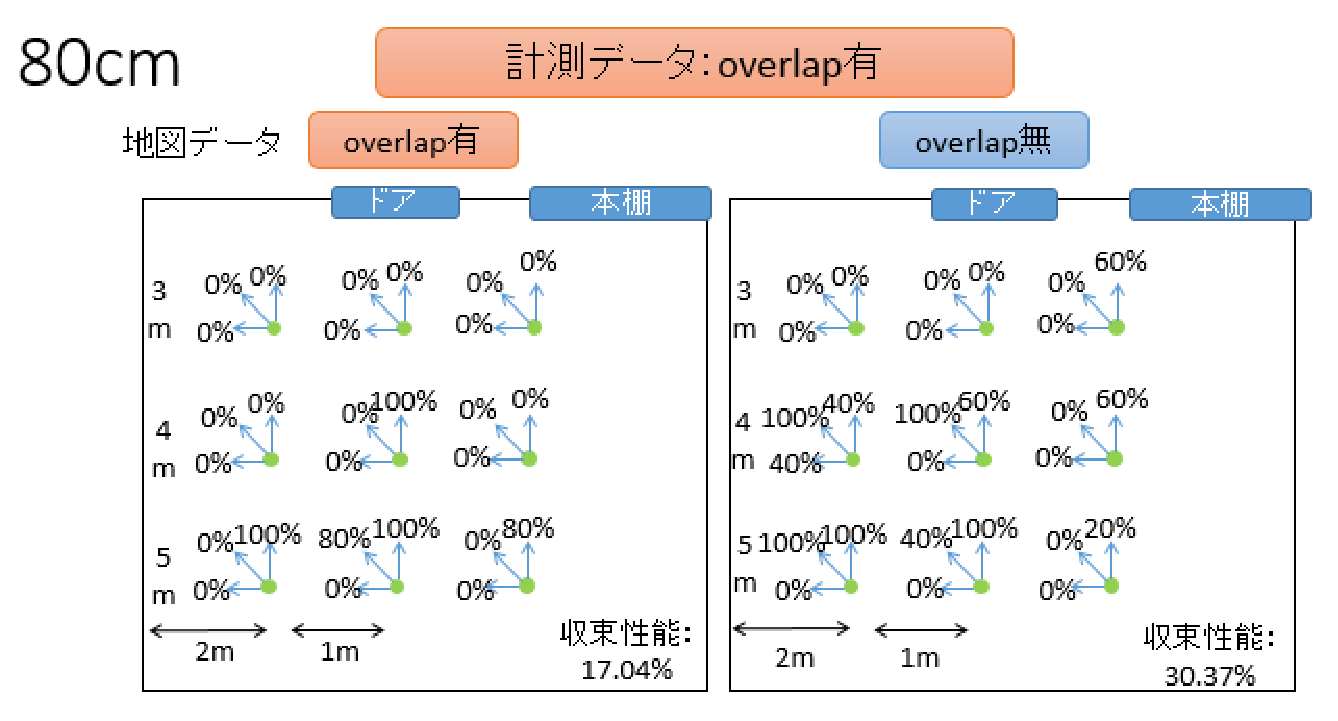
\includegraphics[height=80mm]{figure/有有無.eps}
   \caption{ボクセルサイズ:80cm,計測データオーバーラップ有かつ地図データオーバーラップ有無}
   \label{80-1}
  \end{center}
\end{figure}
%



%
\begin{figure}[htbp]
  \begin{center}
   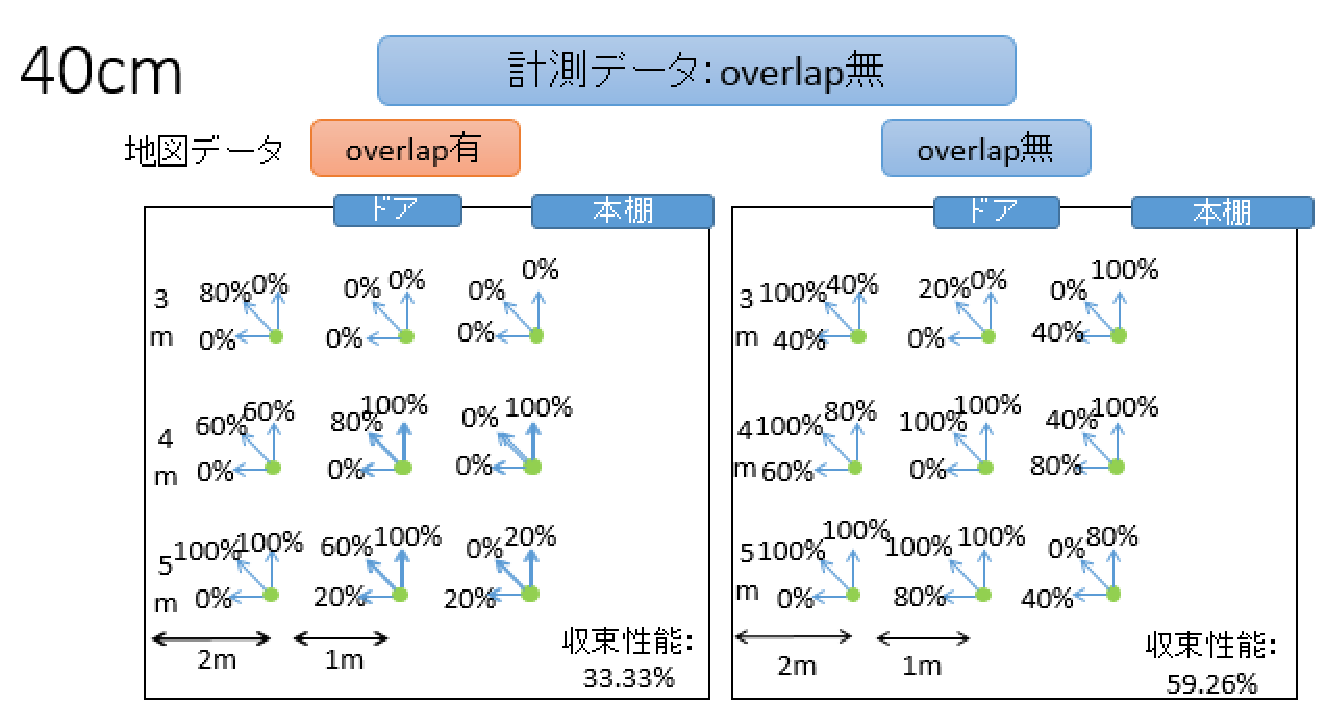
\includegraphics[height=80mm]{figure/無有無2.eps}
   \caption{ボクセルサイズ:40cm,計測データオーバーラップ無かつ地図データオーバーラップ有無}
   \label{40-0}
  \end{center}
\end{figure}
%

%
\begin{figure}[htbp]
  \begin{center}
   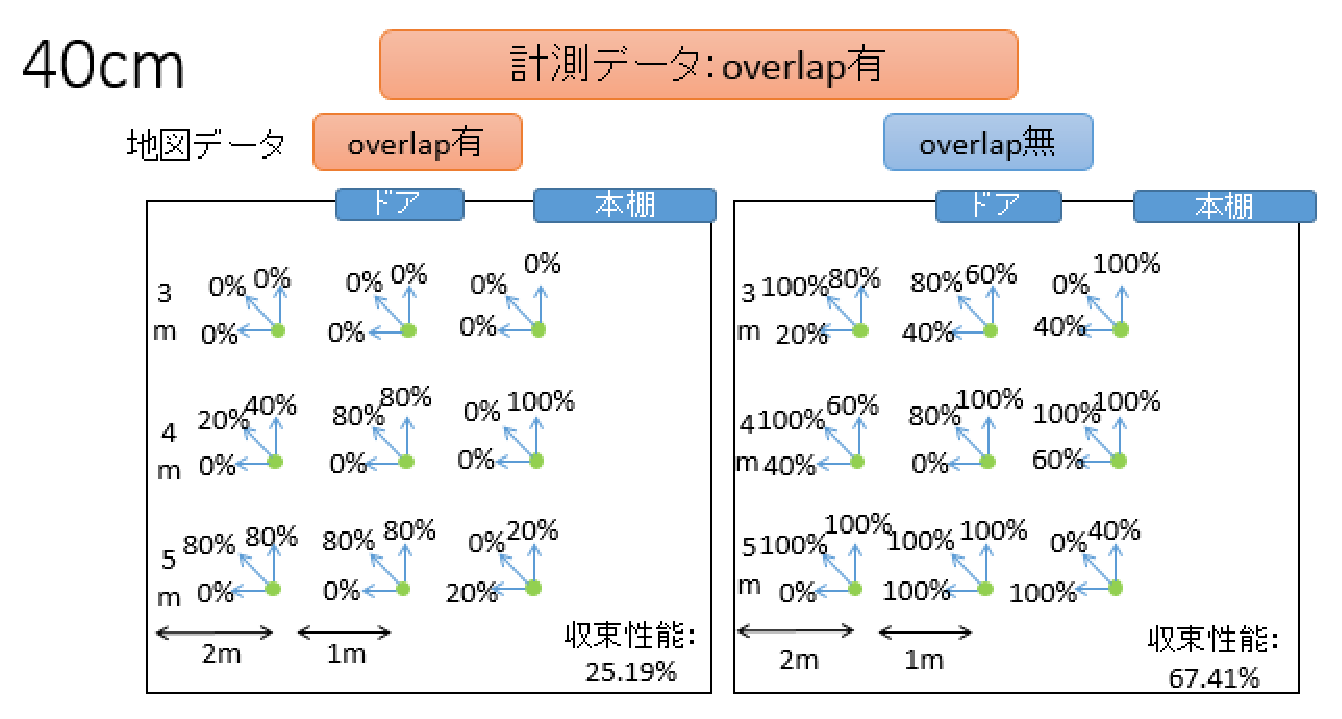
\includegraphics[height=80mm]{figure/有有無2.eps}
   \caption{ボクセルサイズ:40cm,計測データオーバーラップ有かつ地図データオーバーラップ有無}
   \label{40-1}
  \end{center}
\end{figure}
%

\newpage
図4.4~図4.7から見ると,オーバーラップの大きさが80cmの時より40cmの時がより精度が良いことが分かる.これは前述の通り,ボクセルの大きさが小さくなるほど,データの解像度が上がるからである.しかし,ボクセルの大きさが小さくなるほどボクセル数は多くなるため,計算時間が長くなる.また,正面向きの壁から距離が離れるほど精度が良くなるが,その理由は図{\ref{屋内計測データ例}}を見ると距離が離れるほど計測データの量が多くなること,および5mのデータ場合は,角が写っているため,その分距離データが含まれているからである.\par
次に,計算時間について評価する.ただしここでは計算時間の評価は,パーティクル更新時間を用いる.以下に各条件の収束性能とパーティクル更新時間を数値にまとめて表す.収束性能はプログラムを動かしたすべての回数(135回)の中で何回収束されたかを表している.パーティクル更新時間は各条件で最も精度が良かった計測データを使い,その計測データの100回リサンプリングするパーティクル更新時間の平均を取ったものである.

%
\begin{figure}[htbp]
\begin{center}
\begin{tabular}{ccc} \hline
条件 & 収束性能(\%) &  パーティクル更新時間(ms)\\ \hline \hline
80-0-0 & 17.04 & 0.049\\ \hline
80-0-1 & 30.37 & 0.324\\ \hline
80-1-0 & 14.81 & 0.359\\ \hline
80-1-1 & 17.04 & 1.621\\ \hline
40-0-0 & \bf 59.26 & 0.202\\ \hline
40-0-1 & \bf 67.41 & 1.360\\ \hline
40-1-0 & 33.33 & 0.764\\ \hline
40-1-1 & 25.19 & 5.141\\ \hline
\end{tabular}
\end{center}
\end{figure}
%
条件欄の読み方は最初にボクセルの大きさ-地図データのオーバーラップ有無(有:1,無:0)-計測データのオーバーラップ有無(有:1,無:0)である.例えば,80-0-0の場合はボクセルサイズ80cmに地図データオーバーラップ無・計測データオーバーラップ無と同じ意味になる.
上の数値からみると,収束性能が50\%以上で,計算速度が最も早い条件はボクセルサイズ40cmに地図データオーバーラップ無・計測データオーバーラップ無の時である.しかし,精度を一番重視する場合はボクセルサイズ40cmに地図データオーバーラップ無・計測データオーバーラップ有の時である.状況によってパラメータの調整は必要となることが分かる.位置同定行う際のパラメータ条件を以下のようにまとめる.条件毎に収束性能とパーティクル更新時間を比較したグラフが図4.8と図4.9となる.

%
\begin{figure}[htbp]
  \begin{center}
   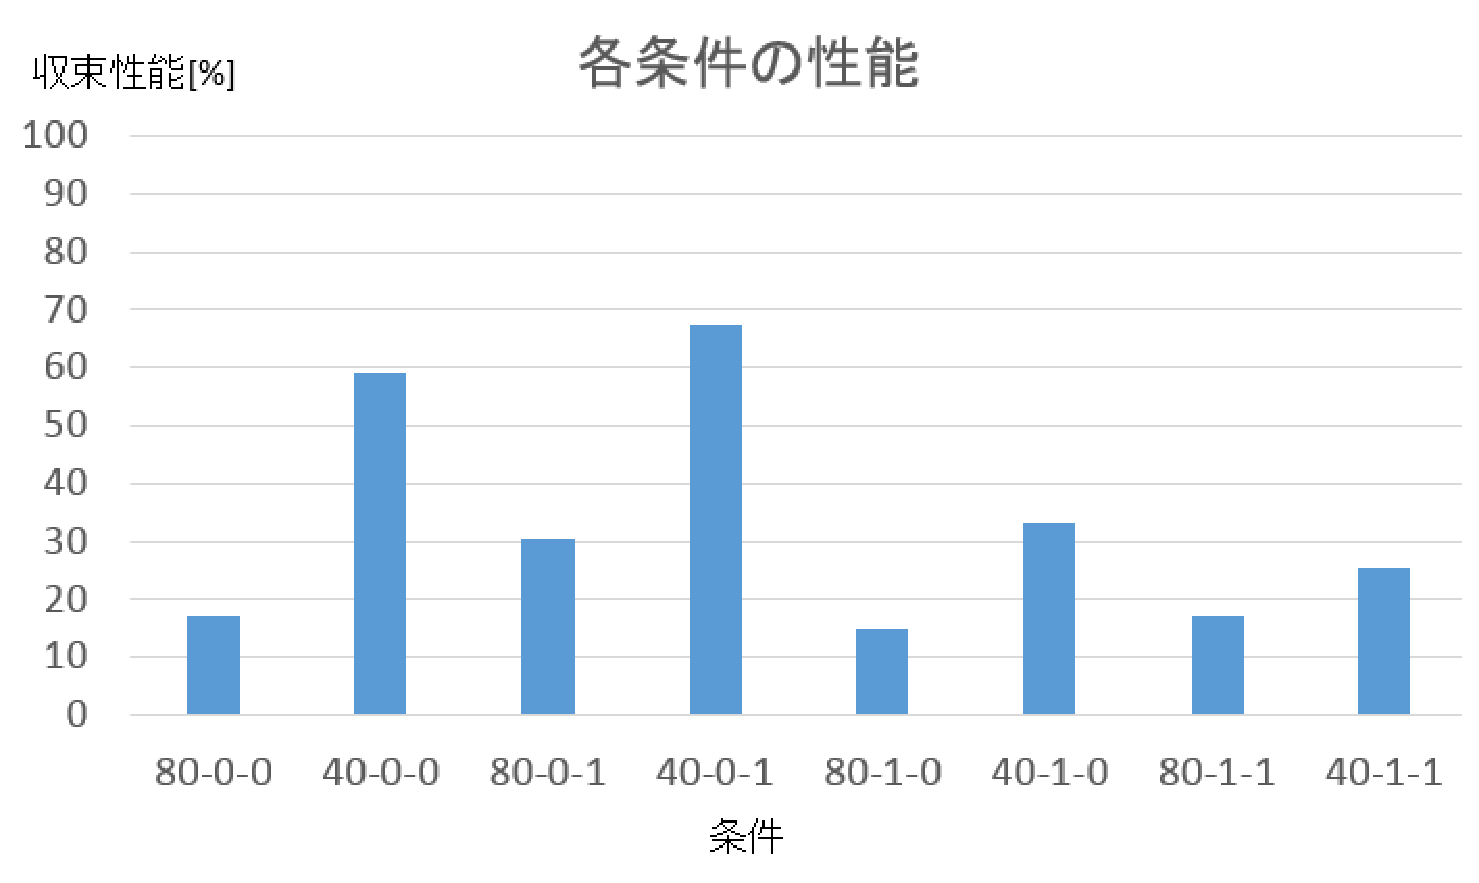
\includegraphics[height=80mm]{figure/各条件の性能.eps}
   \caption{テクスチャー無の各条件の性能}
   \label{各条件の性能}
  \end{center}
\end{figure}
%

%
\begin{figure}[htbp]
  \begin{center}
   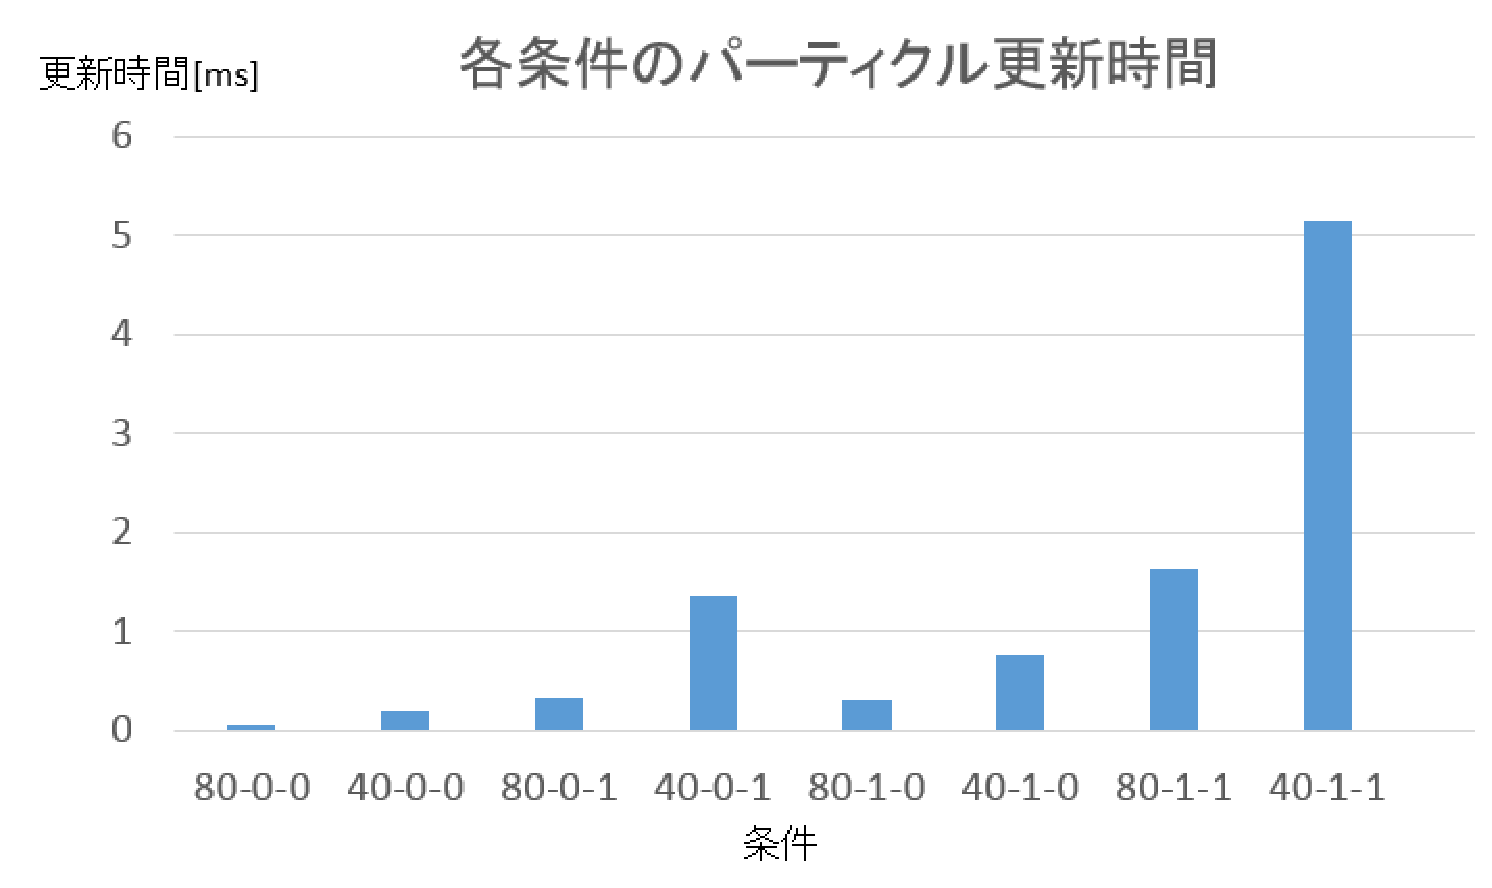
\includegraphics[height=80mm]{figure/各条件のパーティクル更新時間.eps}
   \caption{テクスチャー無の各条件のパーティクル更新時間}
   \label{各条件のパーティクル更新時間}
  \end{center}
\end{figure}
%

\newpage

ボクセルサイズ毎にオーバーラップの有無による収束性能・パーティクル更新時間の比較を見やすくするために以下のようにまとめる.ボクセルサイズ毎の地図データオーバーラップ無・計測データオーバーラップ無の時の収束性能・パーティクル更新時間を各々1とおいて,それに対する条件毎の比例数値を表している.

%
\begin{figure}[htbp]
\begin{center}
\begin{tabular}{ccc} \hline
条件 & 収束性能 &  パーティクル更新時間\\ \hline \hline
80-0-0 & 1 & 1\\ \hline
80-0-1 & 1.783 & 6.623\\ \hline
80-1-0 & 0.870 & 6.243\\ \hline
80-1-1 & 1 & 33.10\\ \hline \hline
40-0-0 & 1 & 1\\ \hline
40-0-1 & 1.138 & 6.734\\ \hline
40-1-0 & 0.563 & 3.789\\ \hline
40-1-1 & 0.425 & 25.46\\ \hline
\end{tabular}
\end{center}
\end{figure}
%
オーバーラップ有無による時間の差は1個のパーティクルに対し周りの8個のボクセルで計算するため計算速度が8倍になる.上の数値からみると,正確に8倍までは及ばないが,計算時間はそれに伴って長くなっていることが確認できる.

\subsection{テクスチャー有の屋内位置同定実験・評価}

次にステレオカメラが認識可能な特徴を増やすため,人為的に作成したテクスチャーを貼った状態で実験を行った.まず,テクスチャー有の屋内実験の様子を図{\ref{テクスチャー有の屋内実験のキャップチャ-}}に表す.次に,作成したテクスチャーを図{\ref{テクスチャー}}に表す.また,テクスチャー有の実験場所をPTX形式にし,MeshLabで見たデータを図{\ref{テクスチャー有の屋内実験場所}}に表す.テクスチャー有の屋内実験は人為的テクスチャーを図{\ref{テクスチャー有の屋内実験場所}}のように壁にA0サイズのテクスチャーを8枚貼った状態で実験を行う.計測する方向は角と壁から3,4,5mの距離から壁向きと角向き2パターンで撮る.テクスチャー有の屋内実験はステレオカメラの特徴認識に最適条件にするため,角向きを撮り,より距離データが含まれるように行う.図{\ref{テクスチャー有の屋内データ例}}にはテクスチャー有の屋内計測データ例を表す.


%
\begin{figure}[htbp]
  \begin{center}
   \includegraphics[height=80mm]{figure/テクスチャー有の屋内実験のキャップチャ-.eps}
   \caption{テクスチャー有の屋内実験の様子}
   \label{テクスチャー有の屋内実験のキャップチャ-}
  \end{center}
\end{figure}
%

\vspace{5mm}
\begin{figure}[htbp]
  \begin{center}
   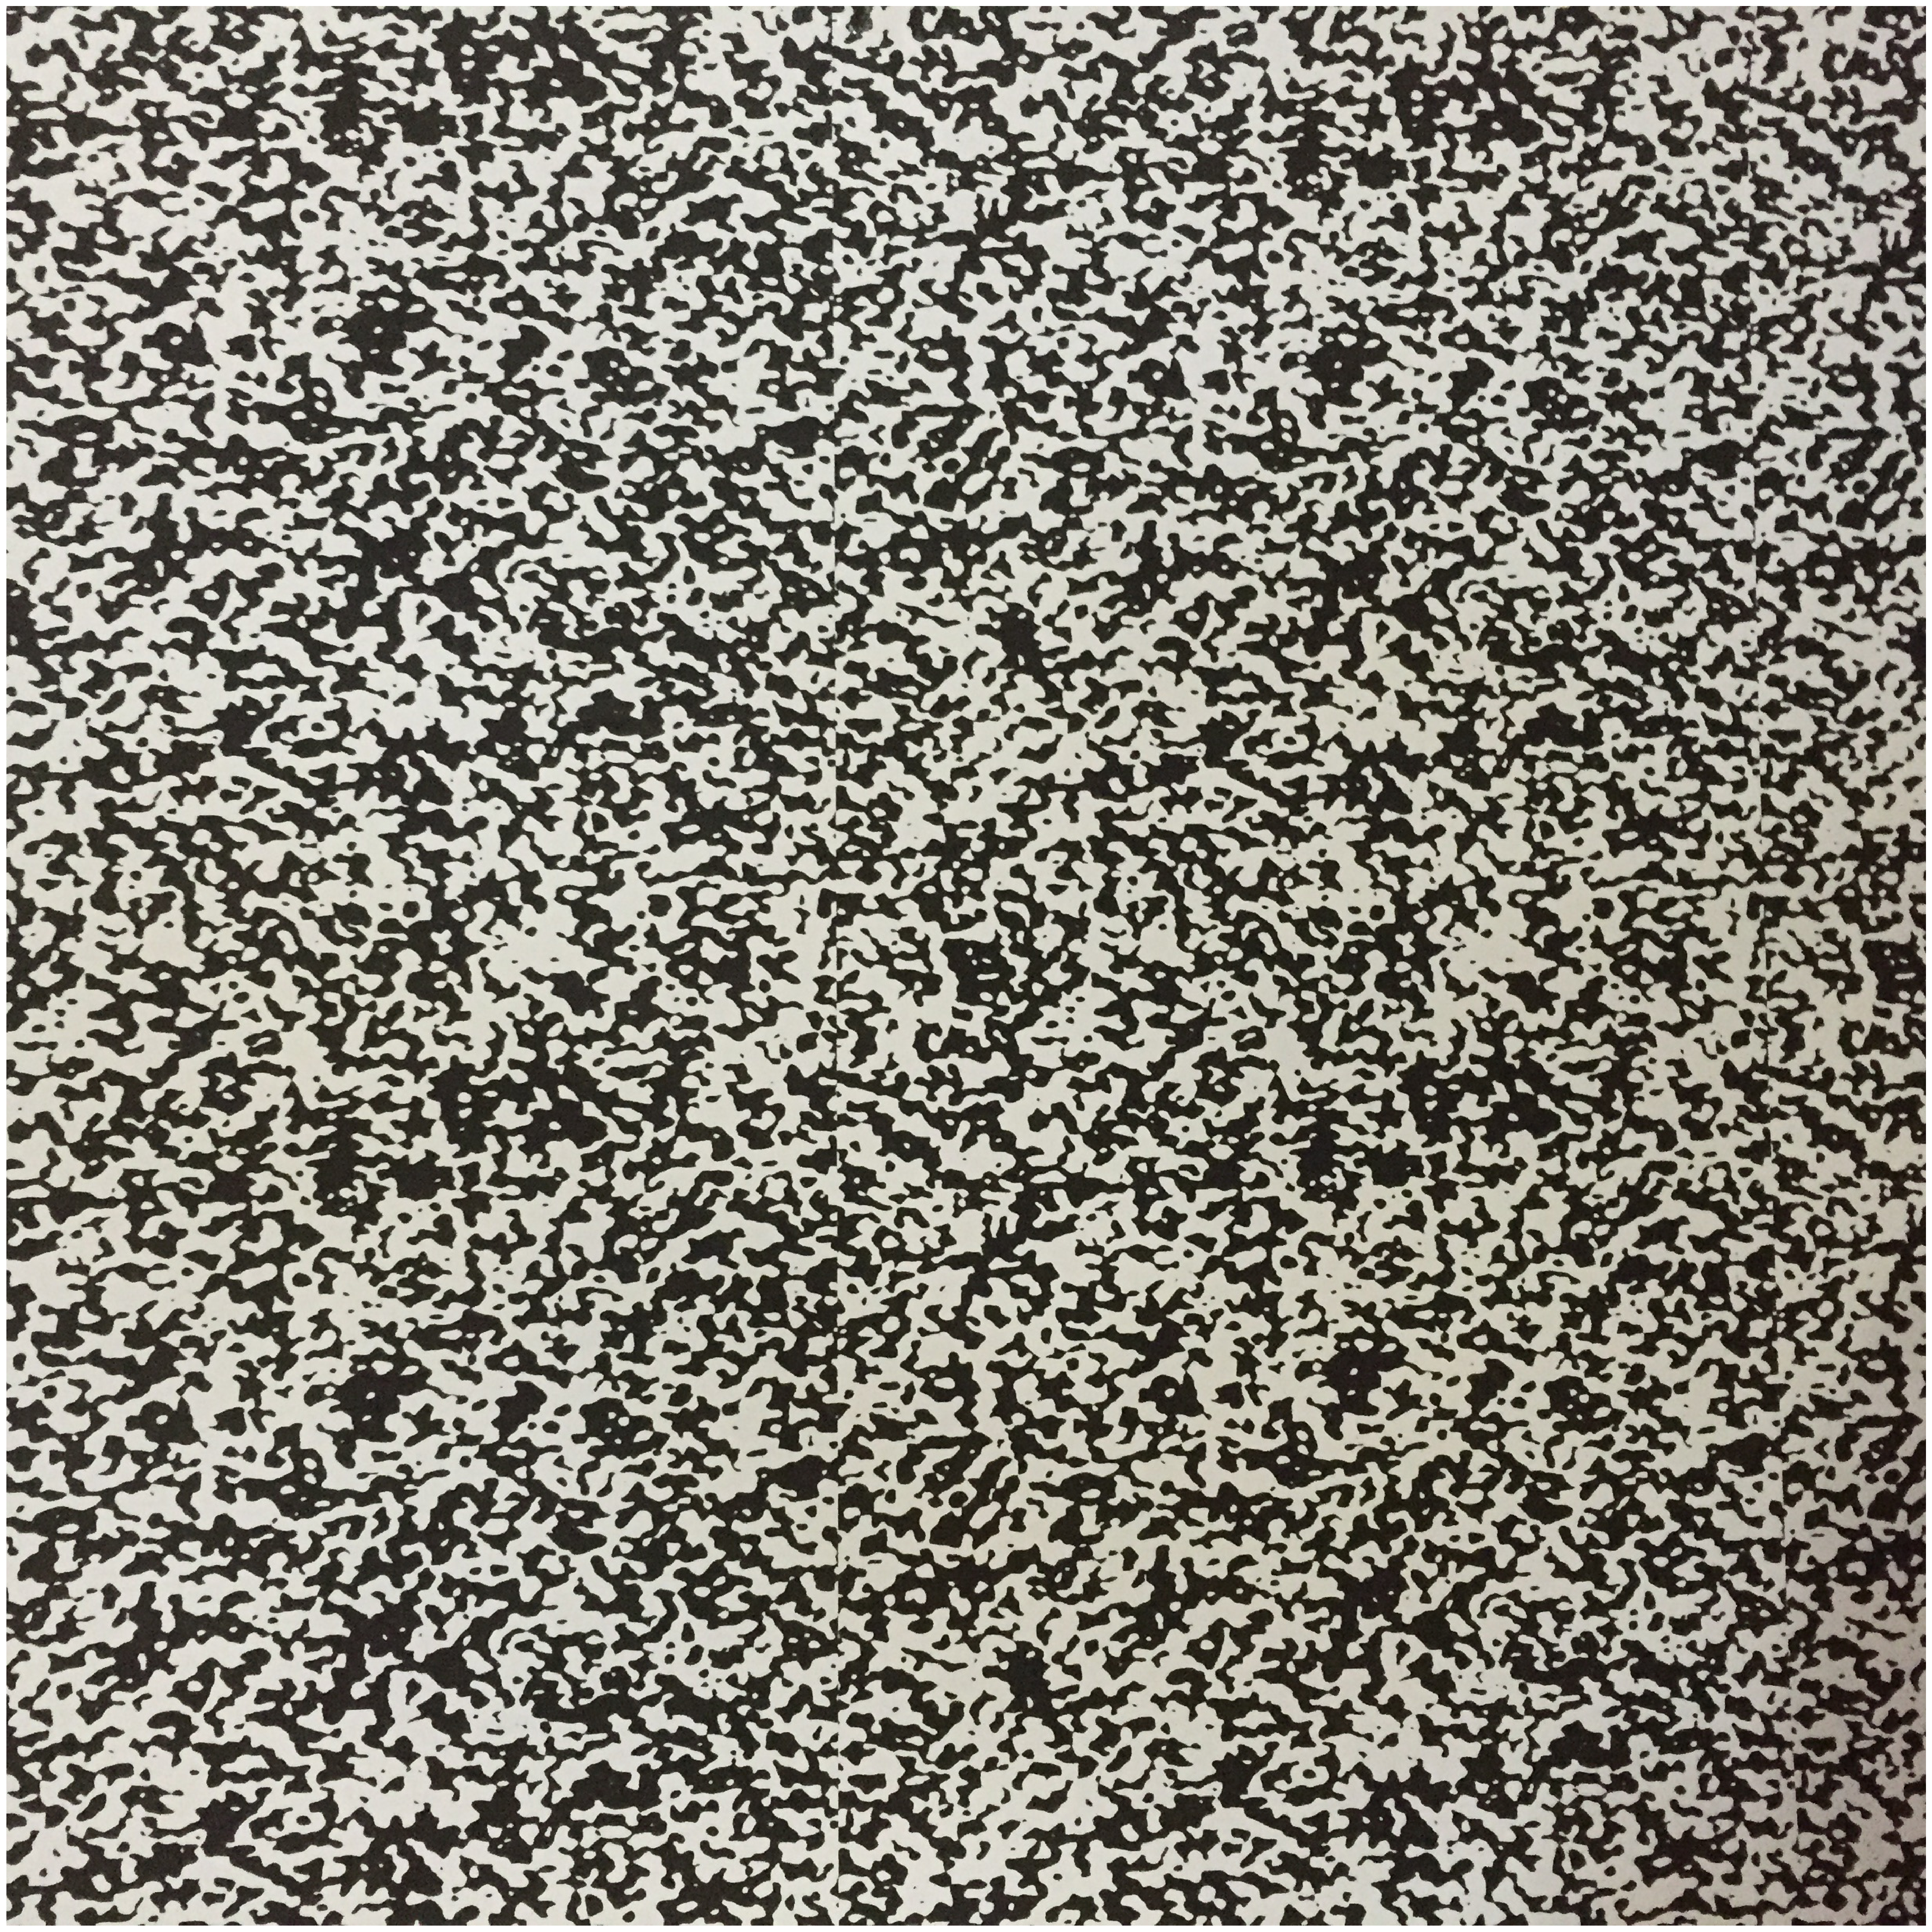
\includegraphics[height=80mm]{figure/テクスチャー.eps}
   \caption{テクスチャー}
   \label{テクスチャー}
  \end{center}
\end{figure}

\begin{figure}[htbp]
  \begin{center}
   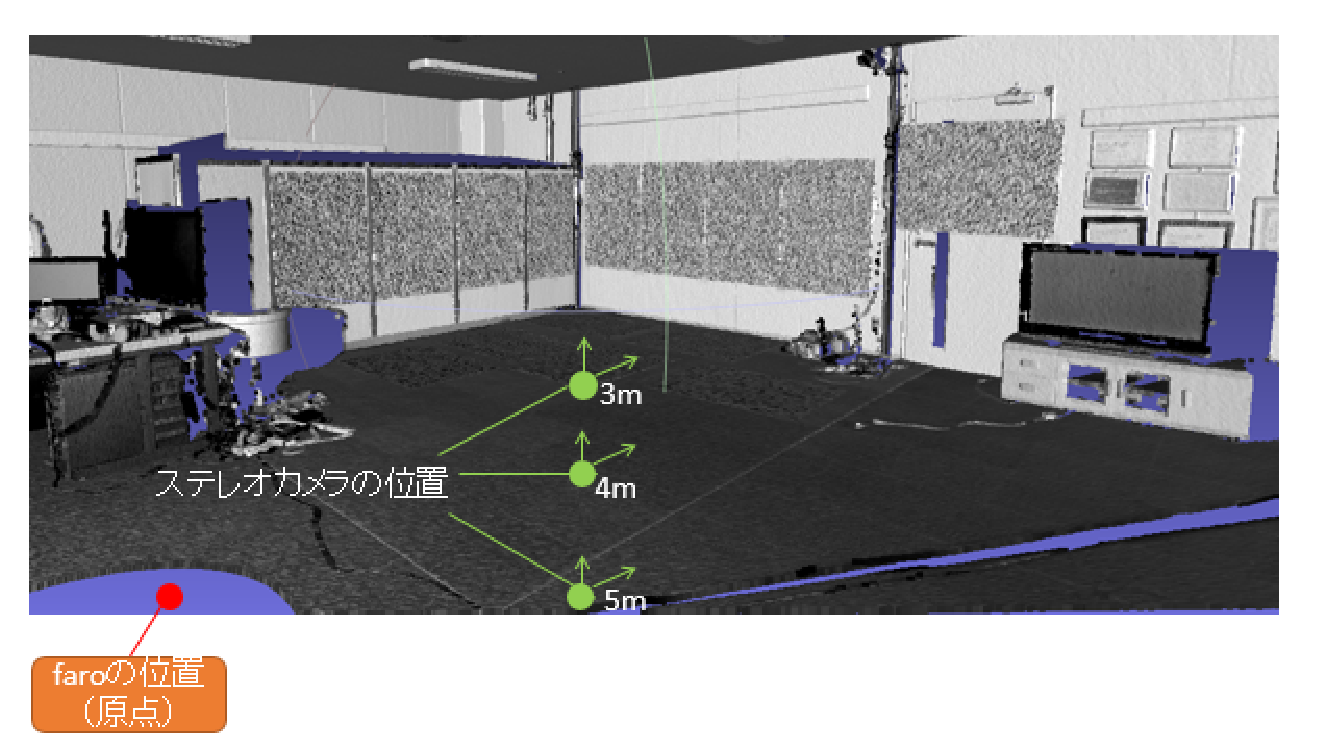
\includegraphics[height=80mm]{figure/テクスチャー有の屋内実験場所.eps}
   \caption{テクスチャー有の屋内実験場所}
   \label{テクスチャー有の屋内実験場所}
  \end{center}
\end{figure}

\begin{figure}[htbp]
  \begin{center}
   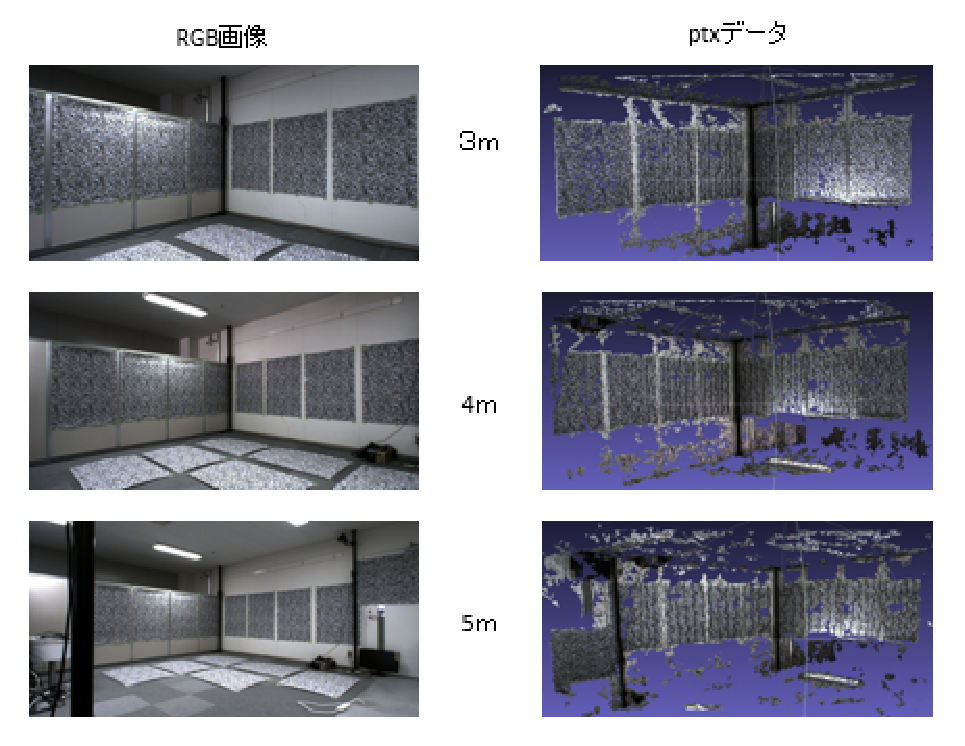
\includegraphics[height=90mm]{figure/テクスチャー有の屋内データ例.eps}
   \caption{テクスチャー有の屋内データ例}
   \label{テクスチャー有の屋内データ例}
  \end{center}
\end{figure}

\vspace{10mm}
テクスチャー有の屋内位置同定実験もテクスチャー無の屋内実験と同様に乱数を与えているため,毎回同じ位置に収束とは限らない.地図データと計測データとの収束性能も5回ずつ繰り返し位置同定を行い,台車の真位置から50cm以内で方向が10°以内の誤差であれば,成功とみなす.パラメータの調整対象もテクスチャー無の時と同様に,ボクセルサイズ80,40cmと地図・計測データのオーバーラップの有無となる.テクスチャー有の屋内位置同定結果をパラメータ毎に図4.14,図4.15に表す.

%
\begin{figure}[htbp]
  \begin{center}
   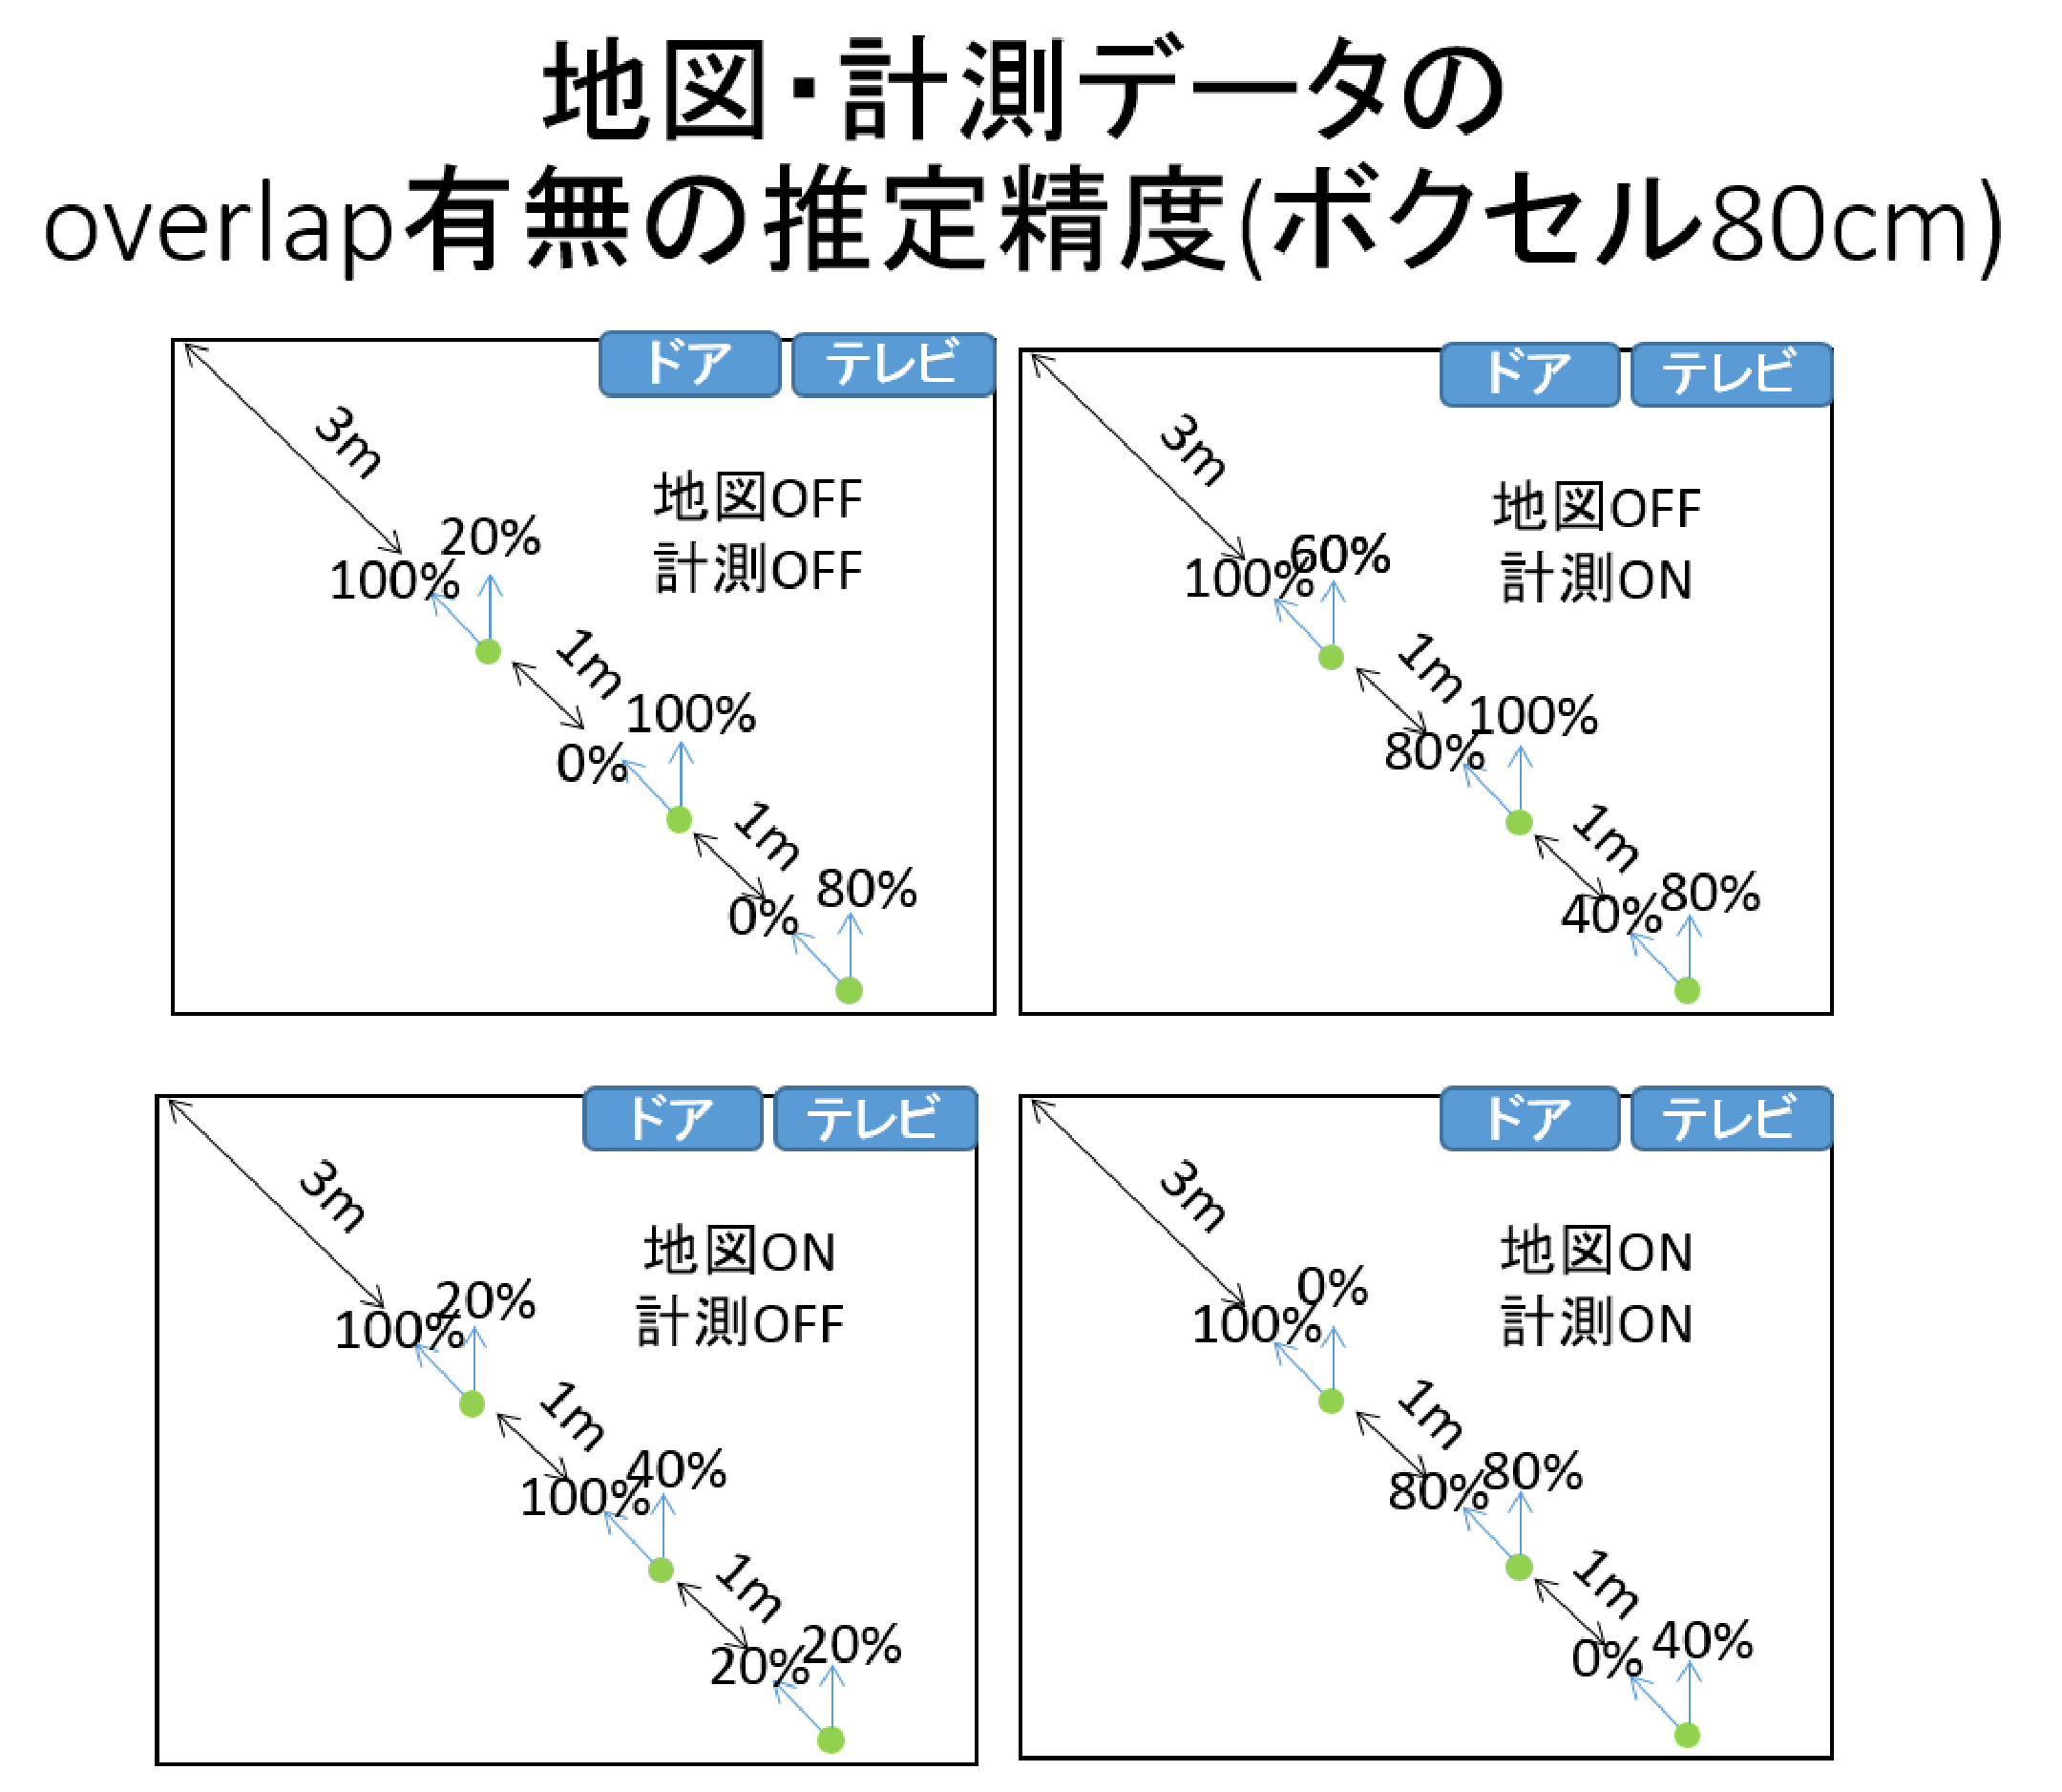
\includegraphics[height=60mm]{figure/有80.eps}
   \caption{テクスチャー有かつボクセルサイズ:80cm}
   \label{80-0}
  \end{center}
\end{figure}
%

%
\begin{figure}[htbp]
  \begin{center}
   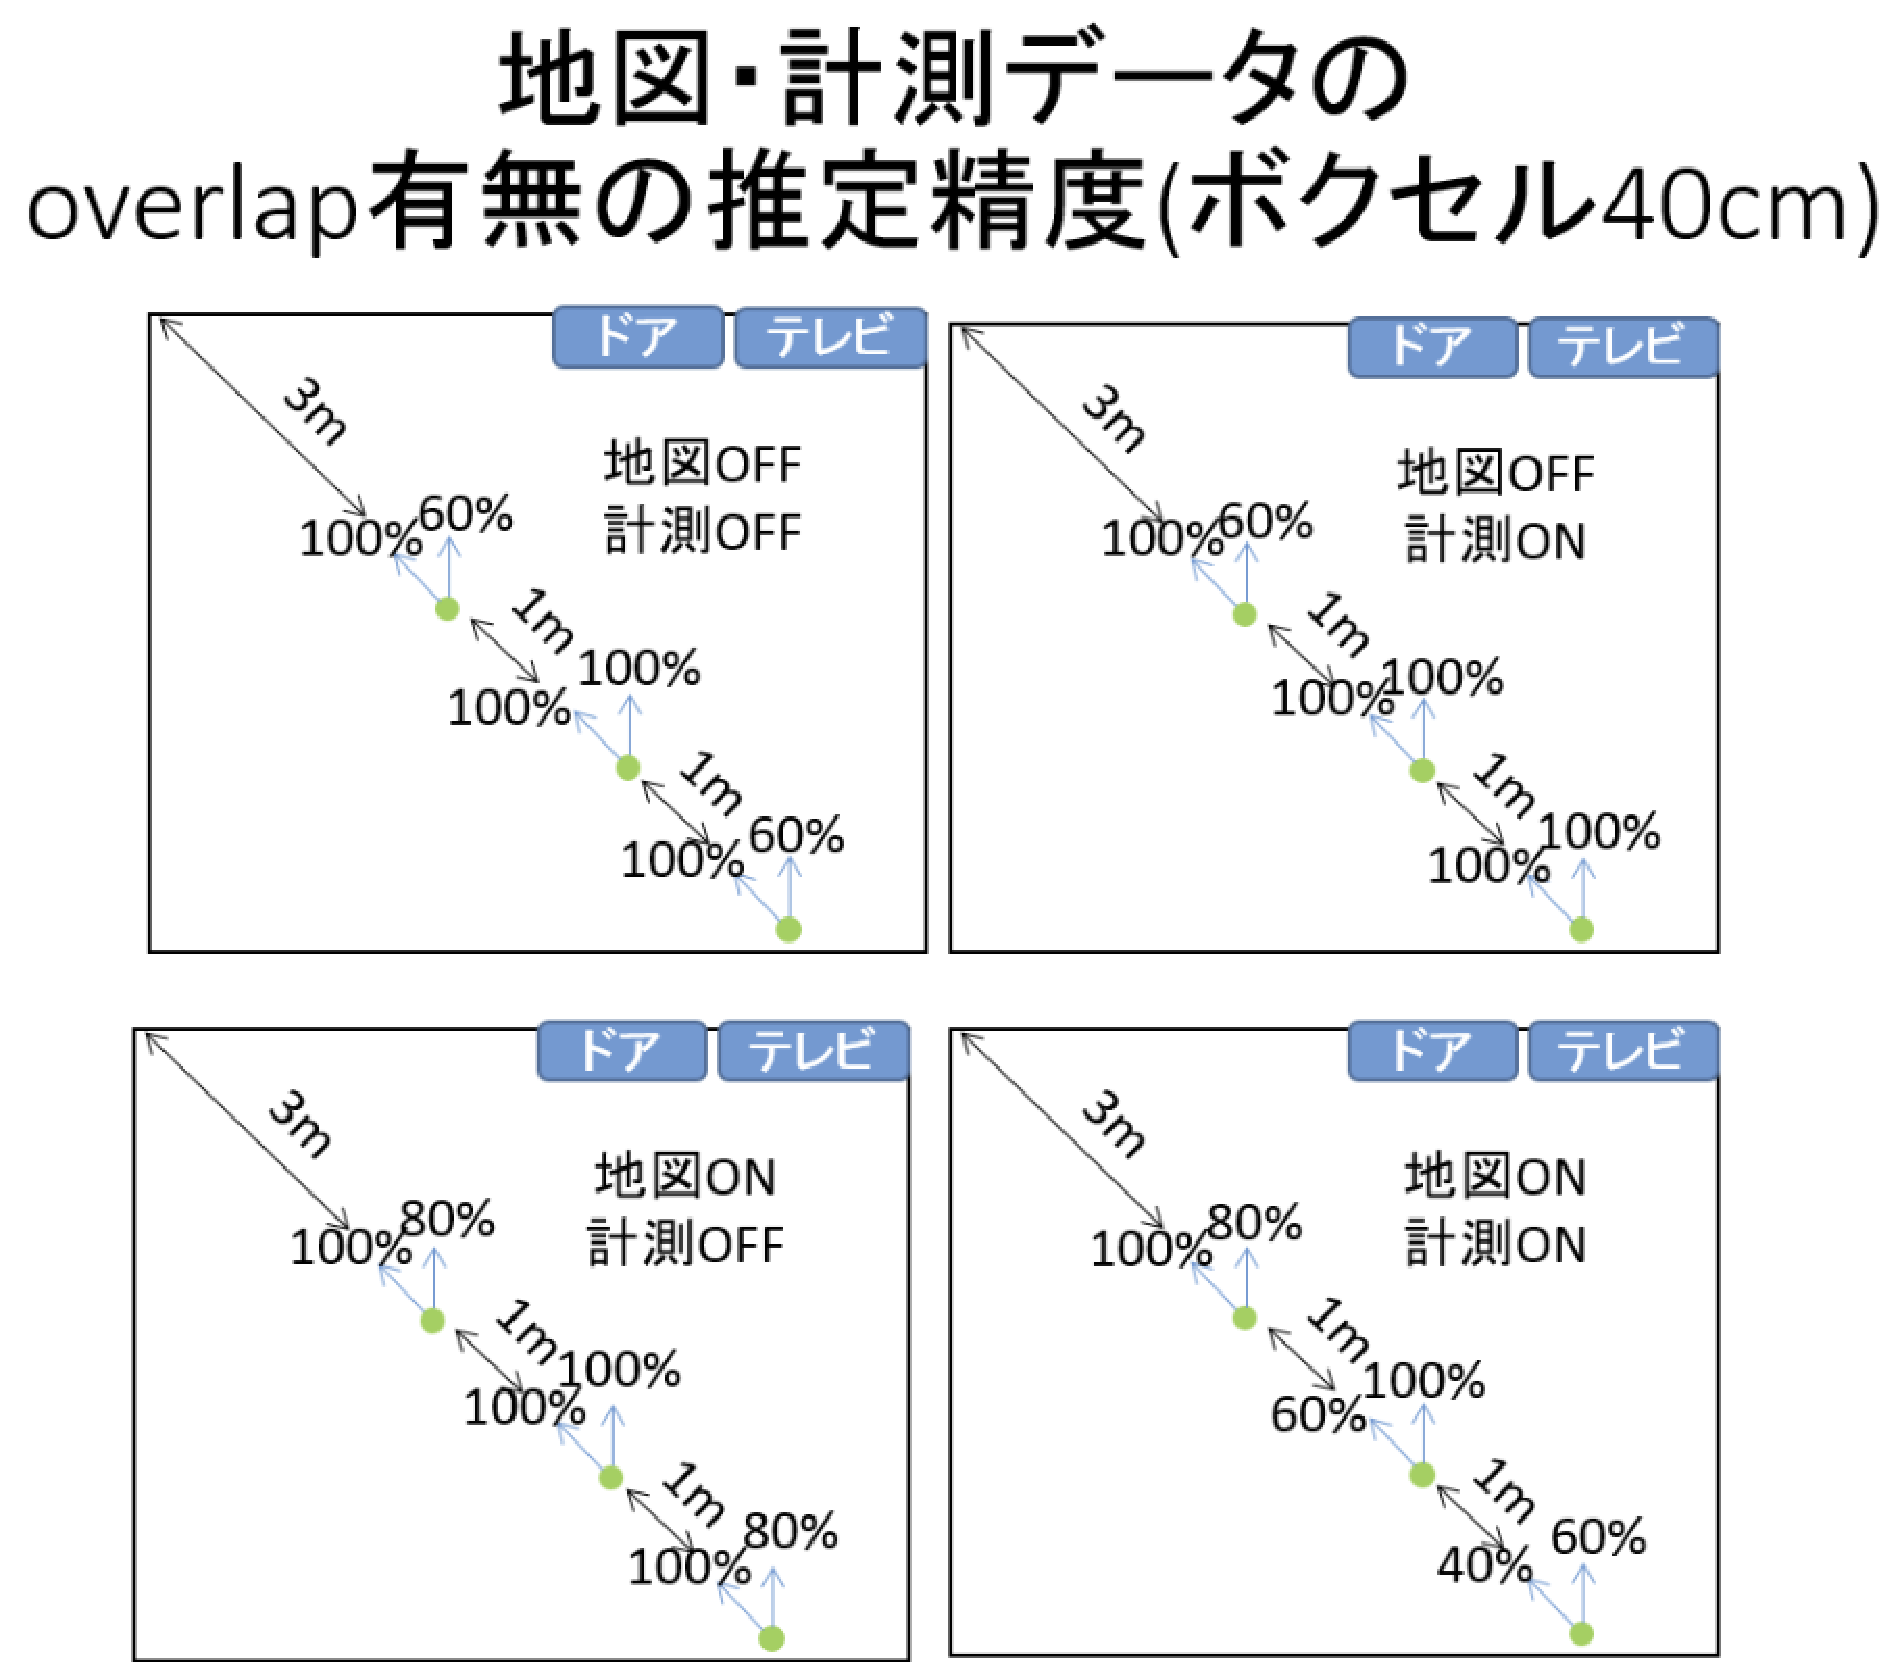
\includegraphics[height=60mm]{figure/有40.eps}
   \caption{テクスチャー有かつボクセルサイズ:40cm}
   \label{80-1}
  \end{center}
\end{figure}
%

\newpage

図4.14と図4.15を見ると,テクスチャー無の結果と同様にボクセルサイズが小さくなると,精度が良くなることが分かる.テクスチャー有の結果を用いてテクスチャー無の結果と同様に,条件毎に収束性能・パーティクル更新時間を数値にまとめた表を以下に表す.

%
\begin{figure}[htbp]
\begin{center}
\begin{tabular}{ccc} \hline
条件 & 収束性能(\%) &  パーティクル更新時間(ms)\\ \hline \hline
80-0-0 & 50 & 0.038\\ \hline
80-0-1 & 66.67 & 0.256\\ \hline
80-1-0 & 50 & 0.166\\ \hline
80-1-1 & 50 & 0.994\\ \hline
40-0-0 & 86.67 & 0.099\\ \hline
40-0-1 & 93.33 & 0.720\\ \hline
40-1-0 & 93.33 & 0.417\\ \hline
40-1-1 & 73.33 & 2.393\\ \hline
\end{tabular}
\end{center}
\end{figure}
%

上のデータから,速度と精度両方重視するのであれば,ボクセルサイズ40cmかつ地図・計測データオーバーラップ無が最も評価が良い.精度だけで比較すると,ボクセルサイズ40cmかつ地図データオーバーラップ無,計測オーバーラップ有が最も評価が良いことが分かる.各条件毎に収束性能・パーティクル更新時間を表したグラフを図4.16と図4.17に表す.\par
テクスチャー無とテクスチャー有のパーティクル更新時間を比較してみると,テクスチャー有の方がパーティクル更新時間が短い.テクスチャー有の方がより,点群がよく撮れているため,ボクセル数が多くてパーティクル更新時間が長いと予測されるが,予測と反対の結果が出ている.その理由と思われるのはデータを撮った場所の違いも挙げられるが,それよりテクスチャー無の方は特徴がばらばらに散らばっているため,ノイズなどを含めた点を計測された点と間違って認識し,無駄なボクセルを作っているためと思われる.実際に同じ条件,ボクセルサイズ80cmかつ地図・計測データオーバーラップ無の時,テクスチャー有のボクセル数は89であった反面,テクスチャー無のボクセル数は184であった.

%
\begin{figure}[htbp]
  \begin{center}
   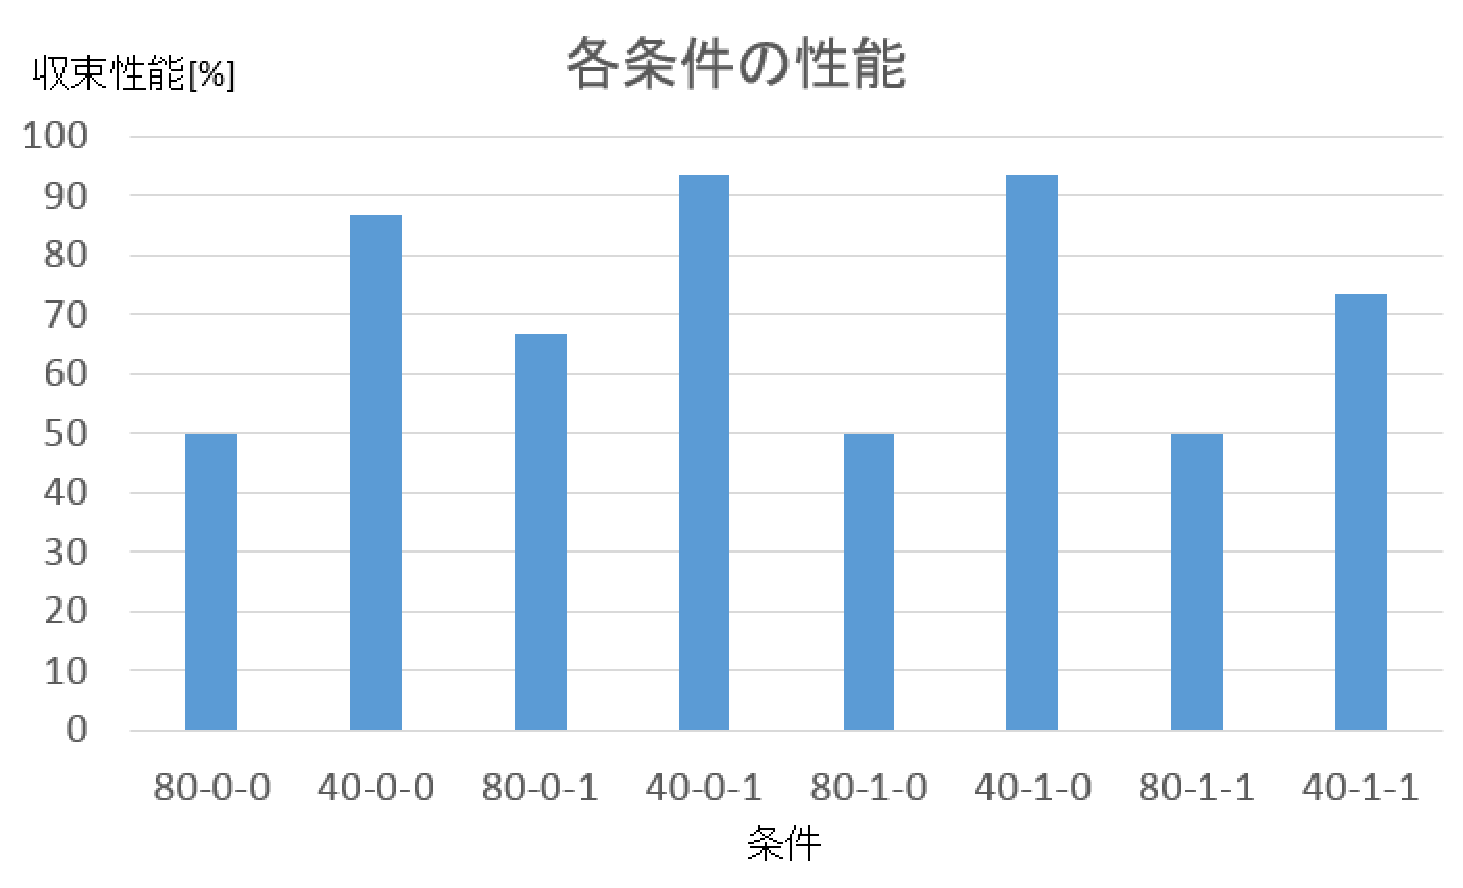
\includegraphics[height=80mm]{figure/各条件の性能2.eps}
   \caption{テクスチャー有の各条件の性能}
   \label{各条件の性能}
  \end{center}
\end{figure}
%

%
\begin{figure}[htbp]
  \begin{center}
   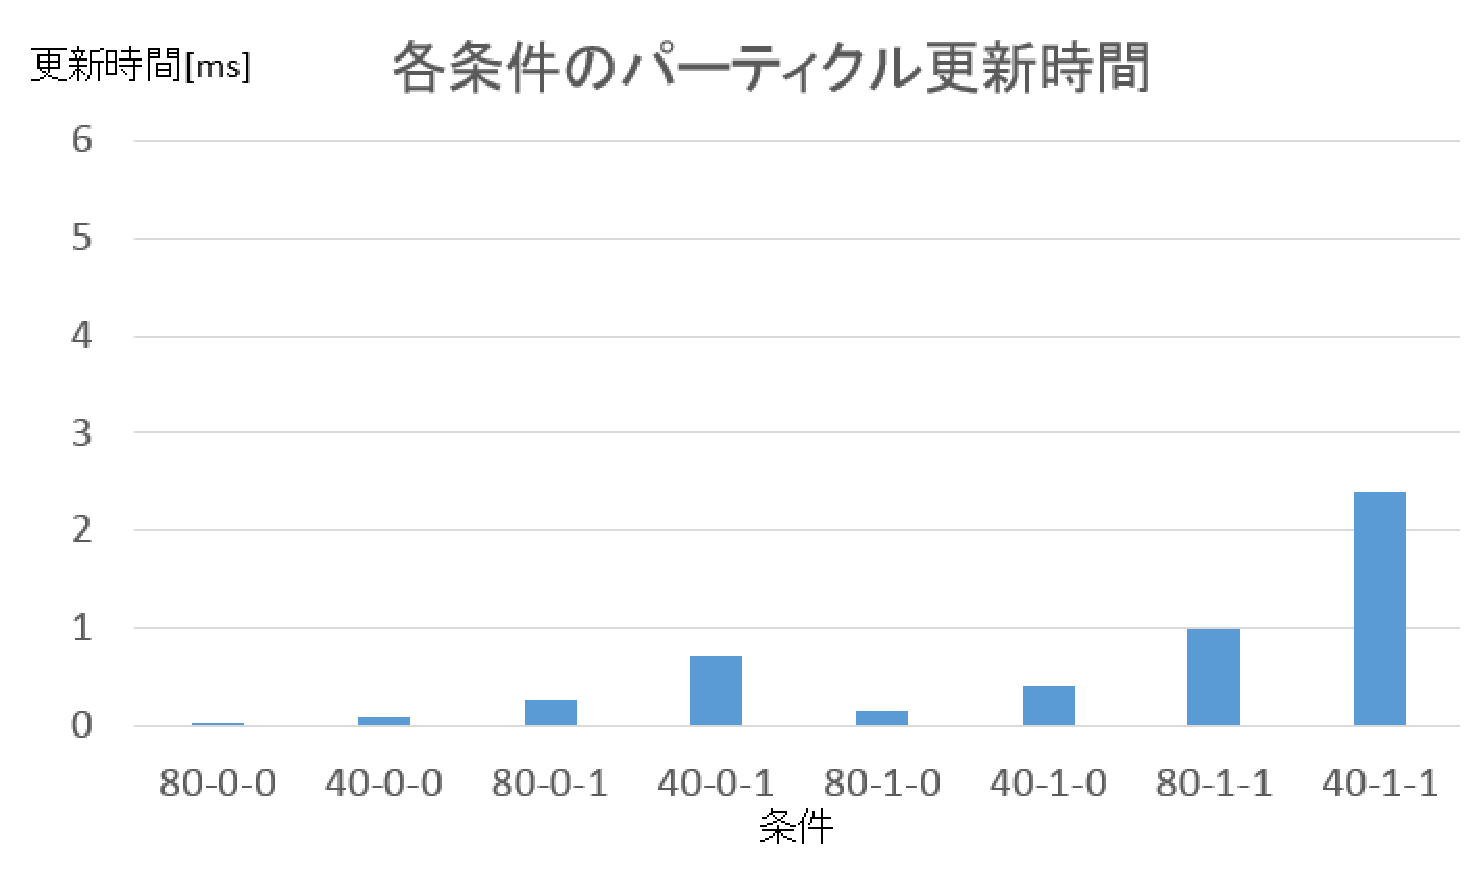
\includegraphics[height=80mm]{figure/各条件のパーティクル更新時間2.eps}
   \caption{テクスチャー有の各条件のパーティクル更新時間}
   \label{各条件のパーティクル更新時間}
  \end{center}
\end{figure}
%

\newpage
上のデータをより比較しやすくするために,ボクセルサイズ毎の地図データオーバーラップ無・計測データオーバーラップ無の時の収束性能・パーティクル更新時間を各々1とおいて,それに対する条件毎の比例数値を以下に表す.

%
\begin{figure}[htbp]
\begin{center}
\begin{tabular}{ccc} \hline
条件 & 収束性能(\%) &  パーティクル更新時間(ms)\\ \hline \hline
80-0-0 & 1 & 1\\ \hline
80-0-1 & 1.333 & 6.650\\ \hline
80-1-0 & 1 & 4.331\\ \hline
80-1-1 & 1 & 25.90\\ \hline \hline
40-0-0 & 1 & 1\\ \hline
40-0-1 & 1.077 & 7.298\\ \hline
40-1-0 & 1.077 & 4.224\\ \hline
40-1-1 & 0.846 & 24.24\\ \hline
\end{tabular}
\end{center}
\end{figure}
%

テクスチャー有無に関係なく,ボクセルサイズによる収束性能・パーティクル更新時間とボクセルサイズに関係なく,テクスチャー有無による収束性能を以下のように表す.左表の収束性能はテクスチャー有無の全てのプログラム実行回数の中,収束された確率で,パーティクル更新時間もテクスチャー有無の全ての条件でのパーティクル更新時間の平均である.右表の収束性能はボクセルサイズ(80,40cm)全てのプログラム実行回数の中で収束された確率である.ボクセルサイズが40cmになると,精度は29.49\%上がる反面,パーティクル更新時間は0.918ms遅くなる.また,テクスチャー有の場合がテクスチャー無の時より精度が37.36\%上がることが分かる.

\begin{table}[htbp]
\begin{center}
\begin{tabular}{|ccc||cc|} \hline
ボクセルサイズ(cm) & 収束性能(\%) &  パーティクル更新時間(ms) & テクスチャー有無 & 収束性能(\%)\\ \hline \hline
80 & 36.99 & 0.469 & 無 & 33.06\\ \hline
40 & 66.48 & 1.387 & 有 & 70.42\\ \hline
差 & 29.49 & 0.918 & 差 & 37.36\\ \hline
\end{tabular}
\end{center}
\end{table}

\newpage

より直感的に性能比較を行うために,収束性能を点数化して評価する.テクスチャー無とテクスチャー有の結果を各シーンで推定精度が80\%以上であれば3点,20\%~60\%であれば1点,0\%であれば0点として,換算した結果をまとめると表4.1と表4.2のようになる.

\begin{table}[htbp]
 \label{Tb:results}
  \begin{center}
    \begin{tabular}{|c|c|c|c|} \hline
	\multicolumn{1}{|c|} {\multirow{2}{*}{地図データ}}
	&\multicolumn{1}{c| }{\multirow{2}{*}{計測データ}}&\multicolumn{2}{c|}{ボクセルサイズ}\\ \cline{3-4}
      & & 40cm & 80cm \\ \hline
	& 有 & 25 & 15 \\ \cline{2-4}
	有 & 無 & 33 & 12 \\ \hline
       & 有 & 55 & 26 \\ \cline{2-4}
      無 & 無 & 49 &16  \\ \hline
    \end{tabular}
\caption{テクスチャー無のオーバーラップ有無による屋内定量評価の結果}
  \end{center}
\end{table}
\begin{table}[htbp]
 \label{Tb:results}
  \begin{center}
    \begin{tabular}{|c|c|c|c|} \hline
	\multicolumn{1}{|c|} {\multirow{2}{*}{地図データ}}
	&\multicolumn{1}{c| }{\multirow{2}{*}{計測データ}}&\multicolumn{2}{c|}{ボクセルサイズ}\\ \cline{3-4}
      & & 40cm & 80cm \\ \hline
	& 有 & 12 & 10 \\ \cline{2-4}
	有 & 無 & 16 & 10 \\ \hline
       & 有 & 16 & 14 \\ \cline{2-4}
      無 & 無 & 14 &10  \\ \hline
    \end{tabular}
 \caption{テクスチャー有のオーバーラップ有無による屋内定量評価の結果}
  \end{center}
\end{table}

テクスチャー有無の関係によらず,ボクセルサイズ400かつ地図データオーバーラップ無,計測データオーバーラップ有の時が最も精度良いが,前の計算時間の結果を考量すると最も有力な設定はボクセルサイズ400かつ地図データオーバーラップ無,計測データオーバーラップ無となる.この結果を踏まえて屋外の位置同定設定はボクセルサイズ400かつ地図データオーバーラップ無,計測データオーバーラップ無の状態とする.

\newpage

\subsection{ステレオカメラとKinect V2との比較実験・評価}
屋内位置同定に優れているKinect V2とステレオカメラを用いた位置同定比較実験を行う.実験場所はステレオカメラの精度が高い環境で実験するため,テクスチャー有の屋内実験場所と同じである.ステレオカメラとKinect V2は同じ台車の上でも図3.16のように違うところに置かれているため,球からKinect V2までの距離を物差しで測り,新しくKinect V2の真位置を求める.求めた真位置とKinect V2の計測データで位置同定を行った収束位置を比較し,収束性能を求める.図{\ref{ステレオカメラとKinectV2計測データ比較}}にステレオカメラとKinect V2の計測データ比較を表す.また,Kinect V2との収束性能を比較する実験のパラメータ設定はテクスチャー有のステレオカメラ収束性能の中で精度が良かったボクセルサイズ40cmかつ地図・計測データオーバーラップ無,ボクセルサイズ40cmかつ地図データオーバーラップ無,計測オーバーラップ有と2パターンにする.

%
\begin{figure}[htbp]
  \begin{center}
   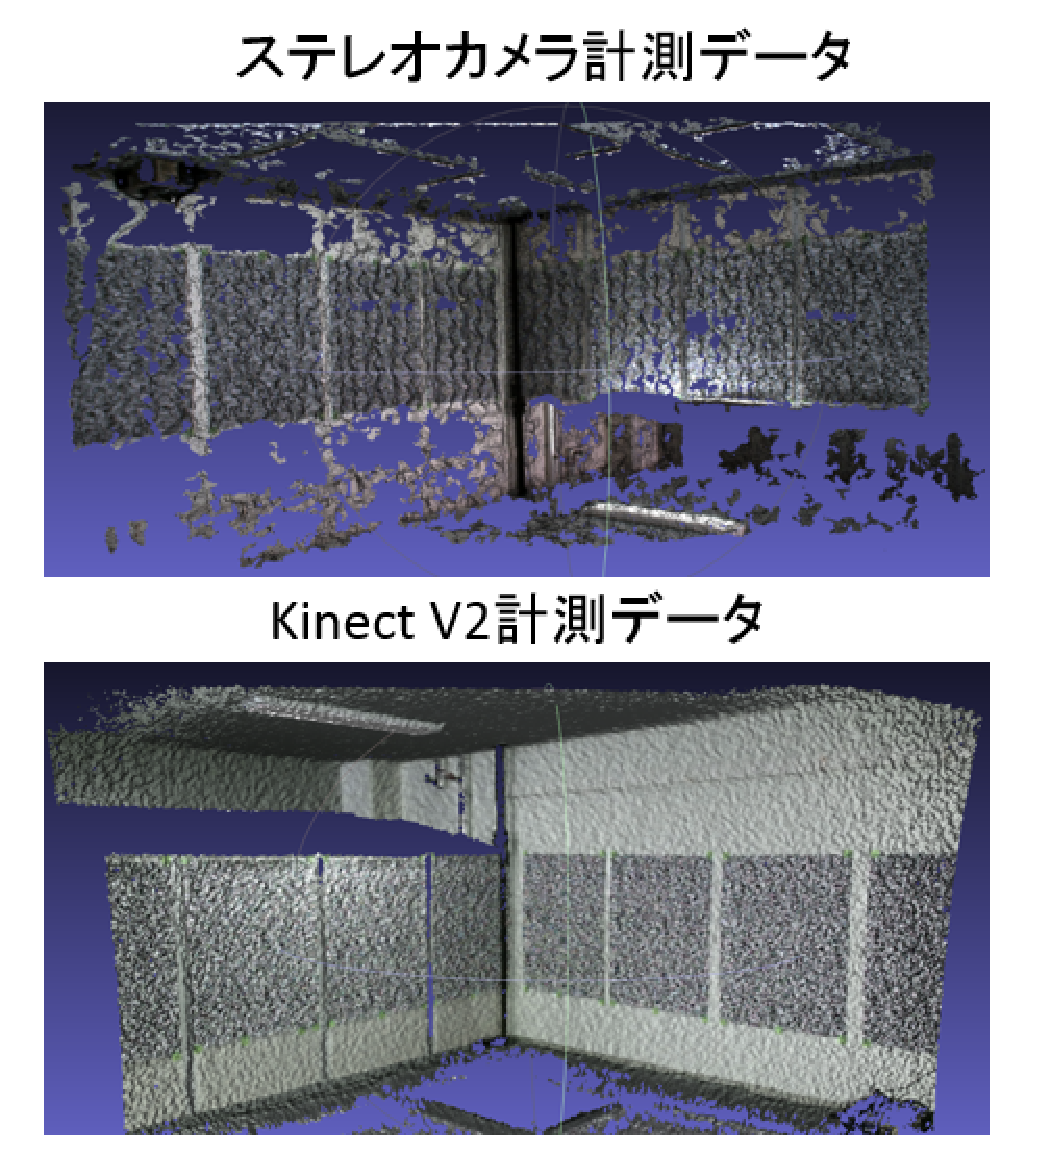
\includegraphics[height=100mm]{figure/ステレオカメラとKinectV2計測データ比較.eps}
   \caption{ステレオカメラとKinectV2計測データ比較例}
   \label{ステレオカメラとKinectV2計測データ比較}
  \end{center}
\end{figure}
%

\newpage

図{\ref{ステレオカメラとKinectV2計測データ比較}}から見ると,ステレオカメラの計測データはノイズが沢山含まれている反面,Kinect V2の計測データは綺麗に撮れていることが分かる.Kinect V2を用いて行った前述した2パターンの収束性能を図4.19に表す.図4.19から見ると,Kinect V2の位置同定精度は100\%である.Kinect V2とステレオカメラの位置同定精度を場所,パラメータ毎にまとめた結果を表4.3と表4.4に表す.

%
\begin{figure}[htbp]
  \begin{center}
   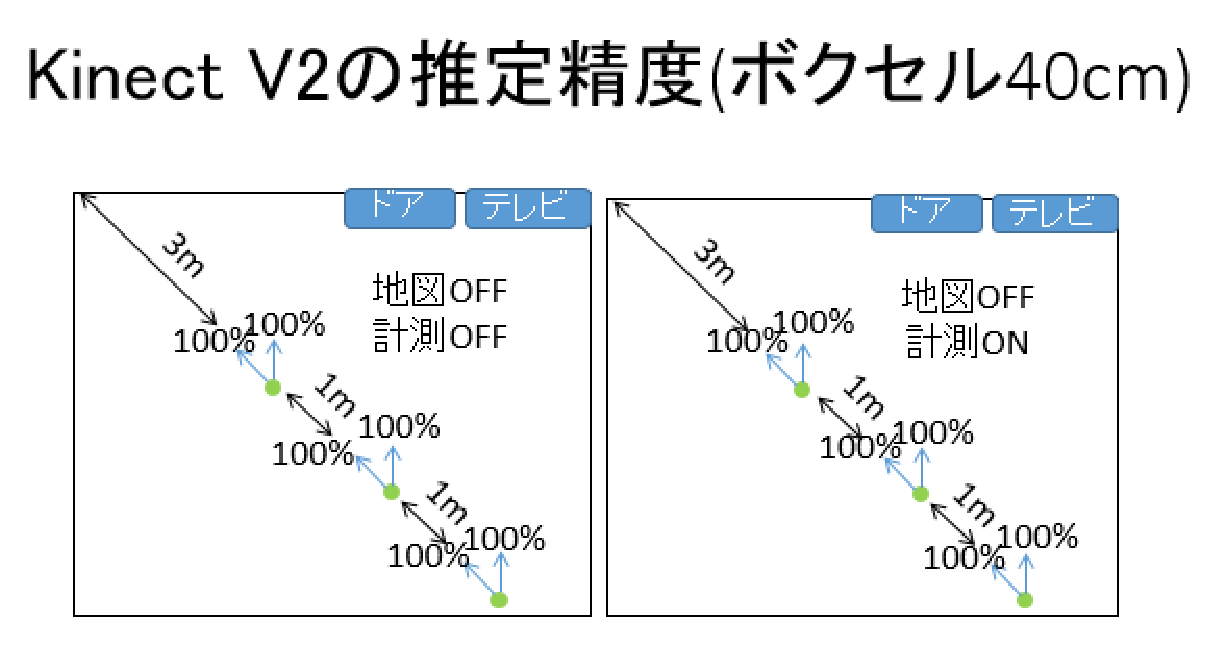
\includegraphics[height=50mm]{figure/KinectV2性能.eps}
   \caption{KinectV2 を用いた場合の収束性能}
   \label{KinectV2性能}
  \end{center}
\end{figure}
%

\begin{table}[htbp]
\begin{center}
\begin{tabular}{|c|c|c|} \hline
正面(m) & Kinect V2推定精度(m) & ステレオカメラの推定精度(m)\\ \hline
3 & 0.165 & 0.605 \\ \hline
4 & 0.110 & 0.202 \\ \hline
5 & 0.120 & 0.567 \\ \hline
平均 & 0.132 & 0.458 \\ \hline\hline
角(m) & Kinect V2推定精度(m) & ステレオカメラの推定精度(m)\\ \hline
3 & 0.112 & 0.108 \\ \hline
4 & 0.134 & 0.068 \\ \hline
5 & 0.148 & 0.105 \\ \hline
平均 & 0.131 & 0.094 \\ \hline
\end{tabular}
\caption{Kinect V2とステレオカメラの位置同定結果比較-ボクセルサイズ40cmかつ地図・計測データオーバーラップ無}
\end{center}
\end{table}

\begin{table}[htbp]
\begin{center}
\begin{tabular}{|c|c|c|} \hline
正面(m) & Kinect V2推定精度(m) & ステレオカメラの推定精度(m)\\ \hline
3 & 0.247 & 0.621 \\ \hline
4 & 0.105 & 0.313 \\ \hline
5 & 0.109 & 0.251 \\ \hline
平均 & 0.154 & 0.395 \\ \hline\hline
角(m) & Kinect V2推定精度(m) & ステレオカメラの推定精度(m)\\ \hline
3 & 0.130 & 0.190 \\ \hline
4 & 0.148 & 0.216 \\ \hline
5 & 0.135 & 0.285 \\ \hline
平均 & 0.138 & 0.230 \\ \hline
\end{tabular}
\caption{Kinect V2とステレオカメラの位置同定結果比較-ボクセルサイズ40cmかつ地図データオーバーラップ無,計測オーバーラップ有}
\end{center}
\end{table}

\newpage

表4.3と表4.4を見ると,ステレオカメラを用いて行う位置同定にはノイズが多く含まれているため,計測データのオーバーラップ有無に関係なく正面向きの壁から3mのところで誤差が大きく生じる.しかし,平均精度の結果を見ると,誤差が1ボクセルの単位である40cm近くであるため,ステレオカメラを用いた屋内の位置同定も,ある程度可能であることが分かる.また,角向きの計測データを用いたステレオカメラによる位置同定はKinect V2の精度にほぼ同じく推定できているため,ステレオカメラを用いた場合の収束性能は十分に高いと考えられる.
\newpage

%---------------------------------------------------------------------------------------------------
\section{屋外実験}
まず,ステレオカメラとRGB-Dカメラの日光の影響による収束性能の比較実験を行った.実験で使われるRGB-DカメラはKinect V2である.ステレオカメラとKinect V2を用いて同じ場所で昼,夕方,夜に分けてデータを撮り,データの比較を行う.次は,屋外位置同定実験・評価である.屋外実環境でステレオカメラを用いて位置同定の精度を確認する.今回屋外で実験を行った場所は九州大学伊都キャンパス図書館前である.最後に,一本の木を3方向から撮り,一本の木の特徴だけでも位置同定可能の有無を確認する実験を行い,評価する.
%---------------------------------------------------------------------------------------------------
\subsection{ステレオカメラとRGB-Dカメラの日光影響によるデータ比較}
まず,ステレオカメラとKinect V2の日光の影響によるデータ比較を行った.まず,計測データを撮った場所を図4.20に表す.実験場所は壁に特徴が多いところであり,距離データを取るため角向きとして行う.

%
\begin{figure}[htbp]
  \begin{center}
   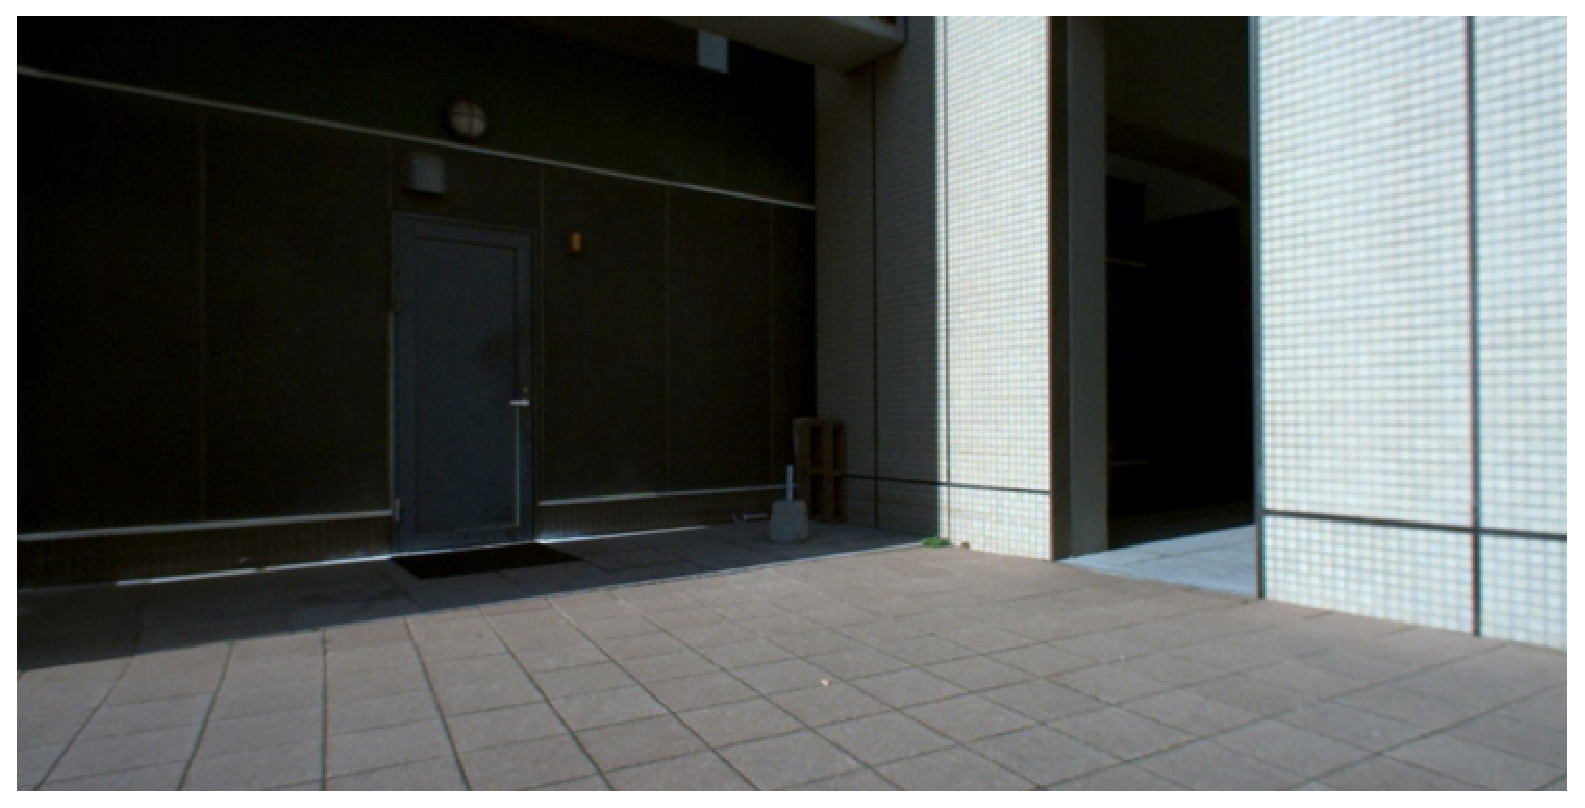
\includegraphics[height=80mm]{figure/日光影響によるデータ比較実実験場所.eps}
   \caption{日光影響によるデータ比較実実験場所}
   \label{日光影響によるデータ比較実実験場所}
  \end{center}
\end{figure}
%

\newpage

図4.20の実験場所で撮った昼,夕方,夜のステレオカメラ,Kinect V2のデータを図4.21に表す.

%
\begin{figure}[htbp]
  \begin{center}
   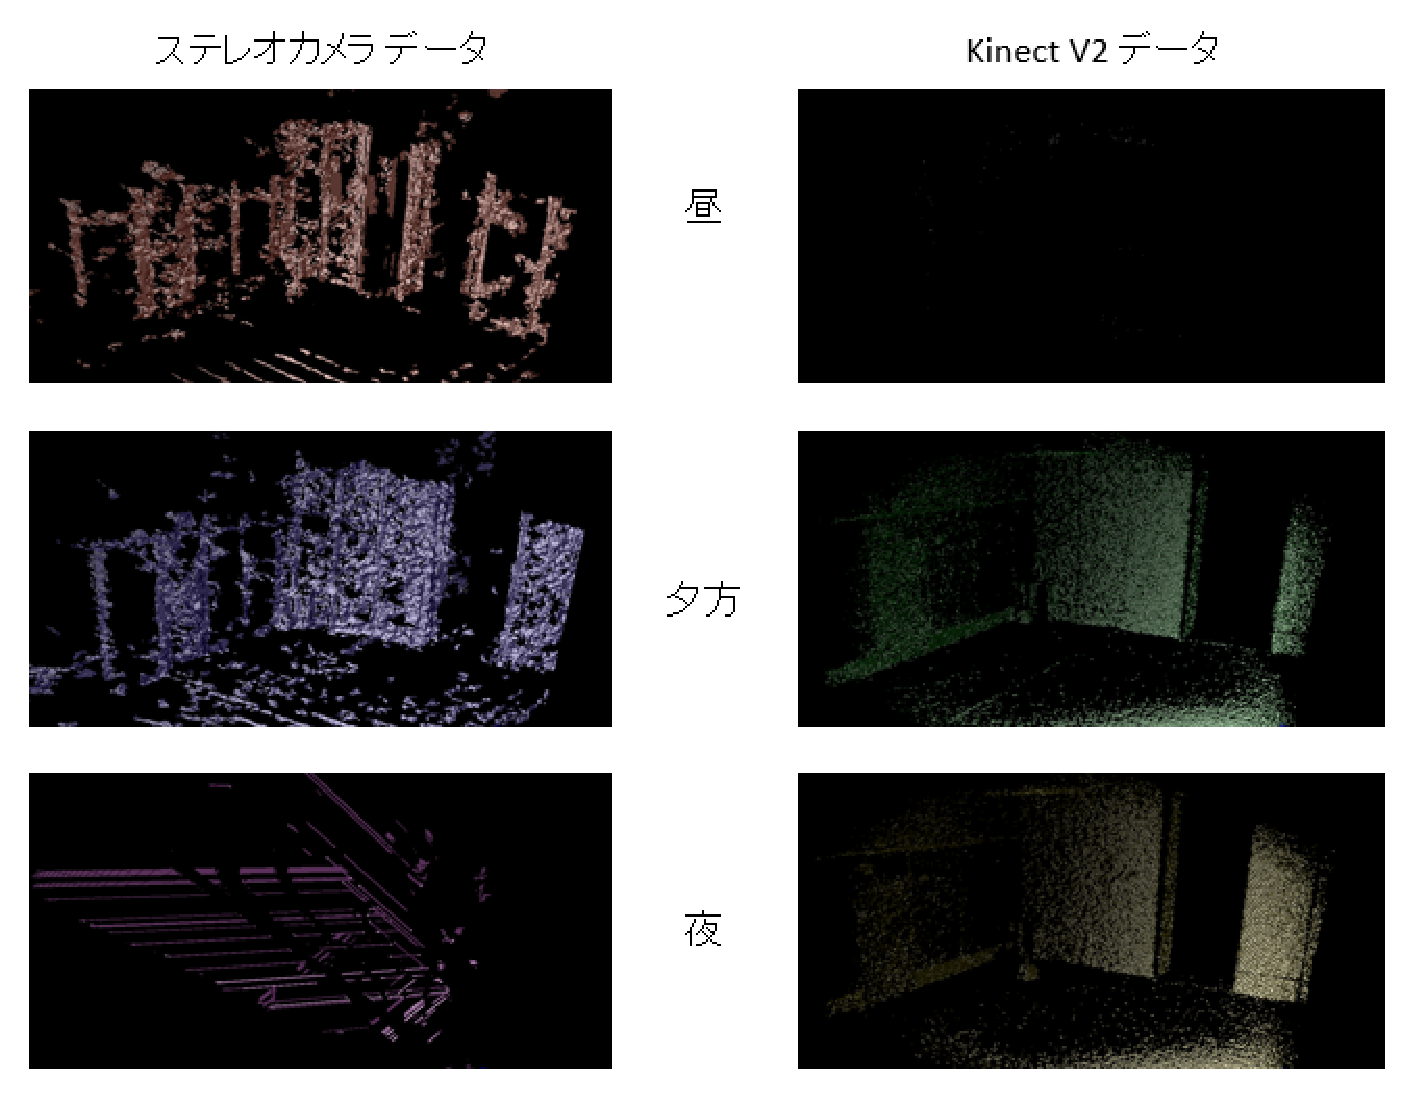
\includegraphics[height=120mm]{figure/日光影響によるデータ比較.eps}
   \caption{日光影響によるデータ比較}
   \label{日光影響によるデータ比較}
  \end{center}
\end{figure}
%

ステレオカメラとKinect V2の日光の影響によるデータ比較をすると,ステレオカメラは日が当たっている時であれば,データが綺麗に撮れている反面,Kinect V2は赤外線を用いたセンサであるため日が当たっているとデータが全然撮れていないことが分かる.しかし,日が沈んでKinect V2のレンズに日が当たっていなければ,Kinect V2データの方がより綺麗に撮れていることが分かる.ステレオカメラの夜データは後ろの壁の隙間から光が出ていたため,図4.21のような結果が出たと思われる.まとめると,屋外の位置同定は昼間や街灯など照明がある状況であれば,日光の影響や計測距離から,ステレオカメラの方がより適していることが分かる.
%---------------------------------------------------------------------------------------------------
\subsection{屋外位置同定実験・評価}
次は屋外の実環境でステレオカメラを用いた位置同定実験を行う.屋外位置同定実験は前述の通り,屋内評価の際に最も精度良くかつ高速なパターンであるボクセルサイズ40cmかつ地図・計測データオーバーラップ無に設定して行う.まず,実験を行った場所を図4.22に表す.\par
%
\begin{figure}[htbp]
  \begin{center}
   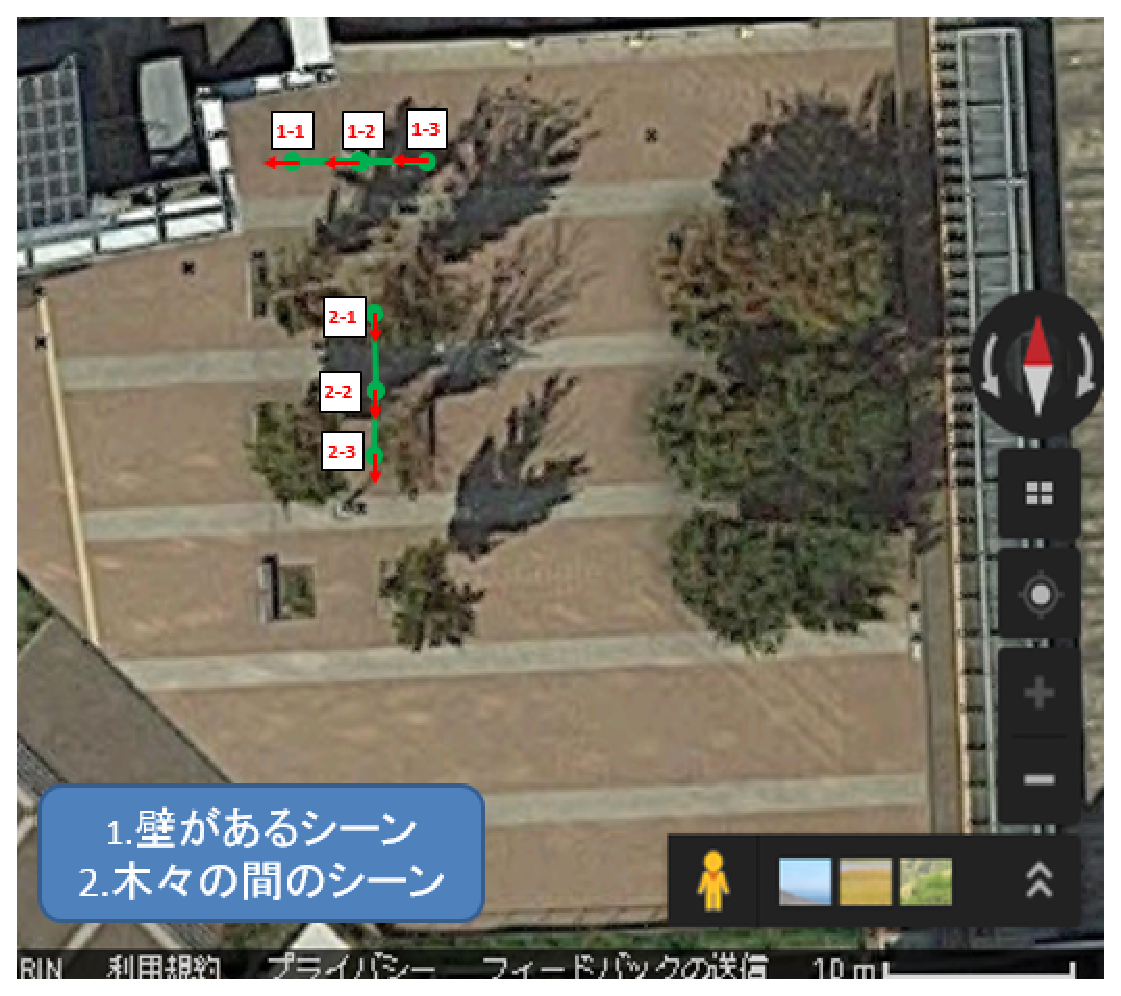
\includegraphics[height=80mm]{figure/屋外実験場所.eps}
   \caption{屋外実験場所}
   \label{屋外実験場所}
  \end{center}
\end{figure}
%
屋外実験を行ったルートは壁があるシーンと木々の間のシーンが撮れるルートの2つである.屋内実験実験とパラメータ条件はほぼ同じであるが,屋外の地図データは屋内に比べるとパーティクルをばら撒く範囲が広いため,台車の真値から半径3m以内にばら撒く範囲を固定して行う.ステレオカメラは性能上距離20mまで撮れるが,ノイズが多く含まれるため,本実験は計測データ10m以上のデータは捨てる.また,位置同定の結果は屋内位置同定と同様に5回繰り返し,x,y,z座標の平均誤差,平均距離誤差,平均方向誤差を各シーン毎に表す.
図4.23は10m以内に壁があるシーン(図4.22中の1-1)の各データを表し,また,表4.5に10m以内に壁があるシーンの位置同定結果を表す.同じく,図4.24には10m以内に壁がないシーン(図4.22中の1-3)の各データを表し,表4.6に10m以内に壁がないシーンの位置同定結果を表す.次は違うルートの木が2つあるシーン(図4.22中の2-1)の各データを図4.25に表し,表4.7に木が2つあるシーンの位置同定結果を表す.最後に,木とポールがあるシーン(図4.22中の2-3)の各データは図4.26に表し,表4.8に木とポールがあるシーンの位置同定結果を表す.


%
\begin{figure}[htbp]
  \begin{center}
   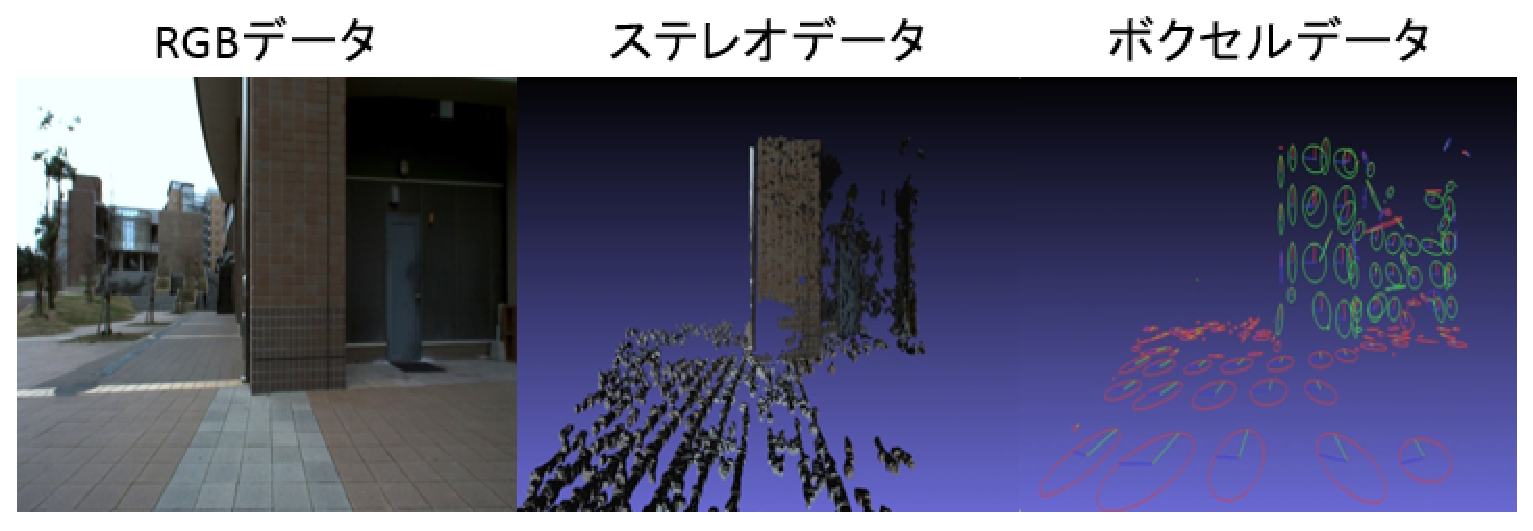
\includegraphics[height=50mm]{figure/10m以内に壁があるシーン.eps}
   \caption{10m以内に壁があるシーンの各データ}
   \label{10m以内に壁があるシーン}
  \end{center}
\end{figure}
%
\begin{table}[htbp]
\begin{center}
\begin{tabular}{|c|c|c|c|c|c|} \hline
\  & x(m) & y(m) & z(m) & 距離(m) & 方向(°)\\ \hline
平均誤差 & 0.08 & 0.17 & 0.08 & 0.21 & 2\\ \hline
\end{tabular}
\caption{10m以内に壁があるシーンの位置同定結果}
\end{center}
\end{table}
%
\begin{figure}[htbp]
  \begin{center}
   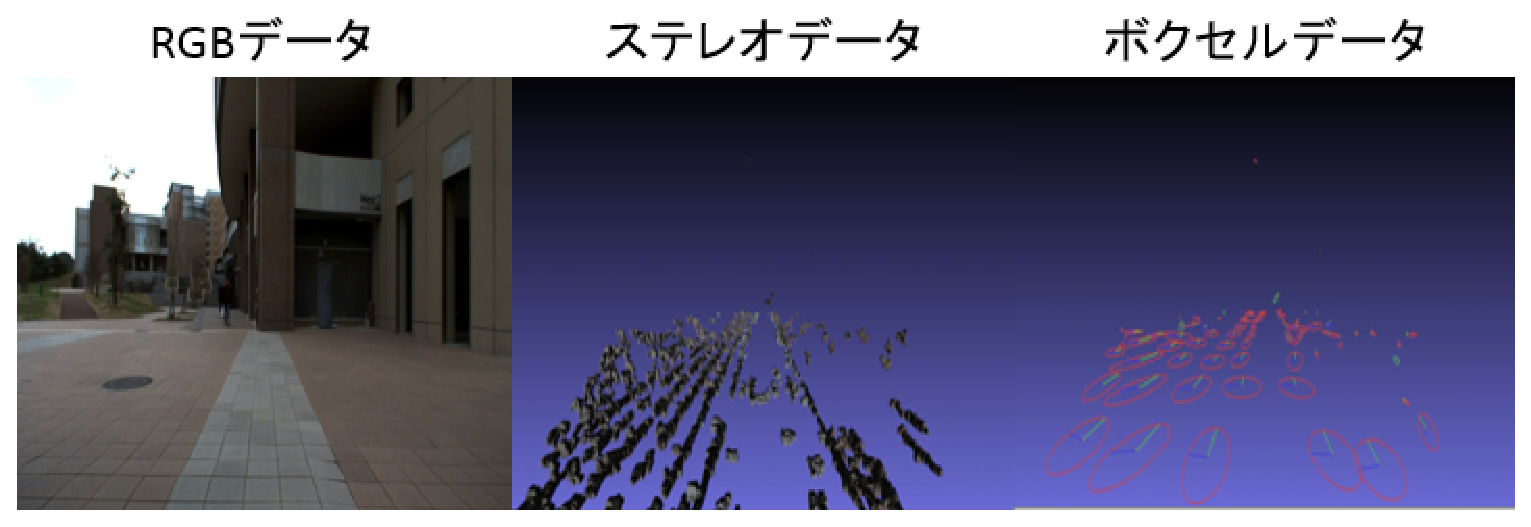
\includegraphics[height=50mm]{figure/10m以内に壁がないシーン.eps}
   \caption{10m以内に壁がないシーンの各データ}
   \label{10m以内に壁がないシーン}
  \end{center}
\end{figure}
%
\begin{table}[htbp]
\begin{center}
\begin{tabular}{|c|c|c|c|c|c|} \hline
\  & x(m) & y(m) & z(m) & 距離(m) & 方向(°)\\ \hline
平均誤差 & 1.22 & 1.81 & 0.00 & 2.31 & 155\\ \hline
\end{tabular}
\caption{10m以内に壁がないシーンの位置同定結果}
\end{center}
\end{table}
%
\begin{figure}[htbp]
  \begin{center}
   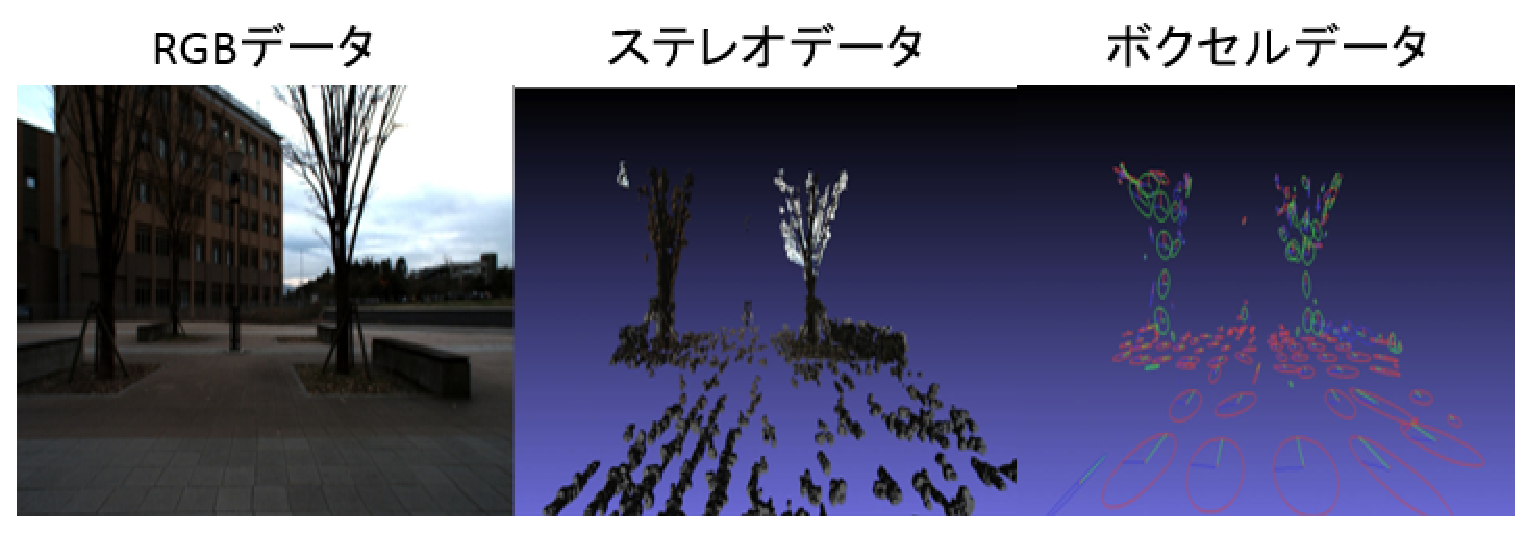
\includegraphics[height=50mm]{figure/木が2つあるシーン.eps}
   \caption{木が2つあるシーンの各データ}
   \label{木が2つあるシーン}
  \end{center}
\end{figure}
%
\begin{table}[htbp]
\begin{center}
\begin{tabular}{|c|c|c|c|c|c|} \hline
\  & x(m) & y(m) & z(m) & 距離(m) & 方向(°)\\ \hline
平均誤差 & 0.34 & 0.13 & 0.08 & 0.38 & 2.6\\ \hline
\end{tabular}
\caption{木が2つあるシーンの位置同定結果}
\end{center}
\end{table}
%
\begin{figure}[htbp]
  \begin{center}
   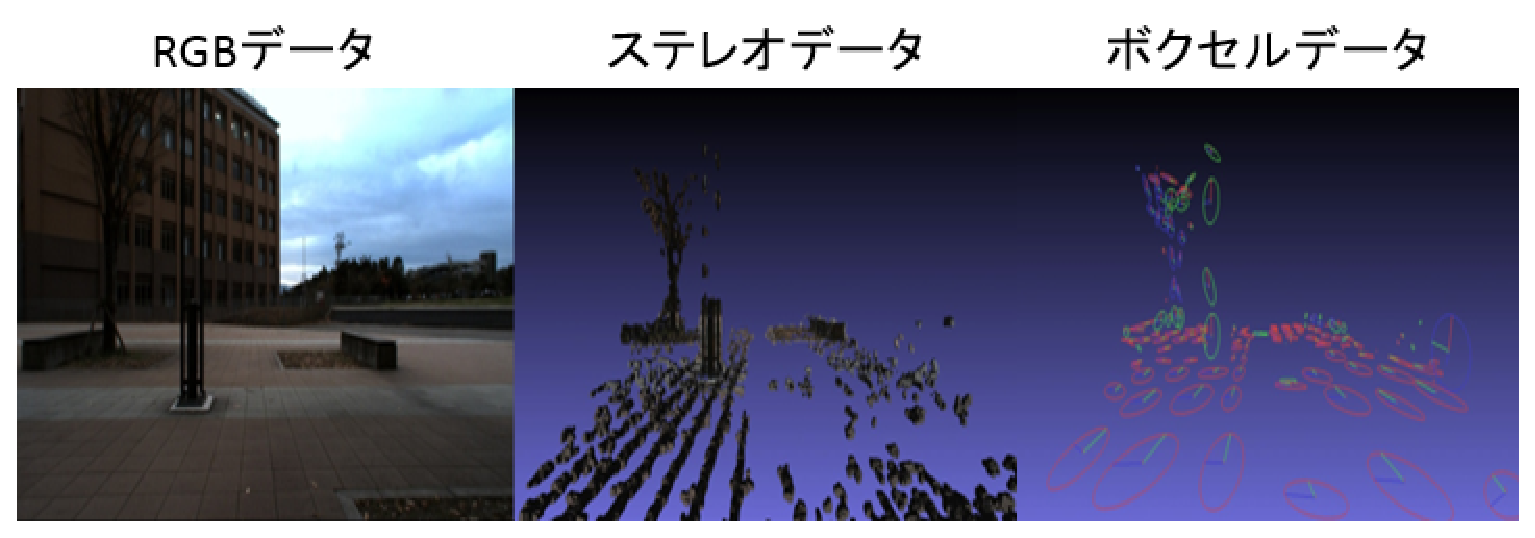
\includegraphics[height=50mm]{figure/木とポールがあるシーン.eps}
   \caption{木とポールがあるシーンの各データ}
   \label{木とポールがあるシーン}
  \end{center}
\end{figure}
%
\begin{table}[htbp]
\begin{center}
\begin{tabular}{|c|c|c|c|c|c|} \hline
\  & x(m) & y(m) & z(m) & 距離(m) & 方向(°)\\ \hline
平均誤差 & 1.24 & 1.68 & 0.09 & 2.1 & 156\\ \hline
\end{tabular}
\caption{木とポールがあるシーンの位置同定結果}
\end{center}
\end{table}
%

\newpage

図4.23の10m以内に壁があるシーンのステレオデータとボクセルデータから見ると,10m以内に壁のテクスチャーがあることと地面のテクスチャーも綺麗に撮れているため,平均誤差が小さい.しかし,図4.24の10m以内に壁がないシーンのデータを見ると,地面のテクスチャーだけで位置同定することになるため,平均誤差の結果から位置同定が難しいことが分かる.図4.25の木が2つあるシーンは2つの木と地面の特徴が撮れているため,このシーンに対する位置同定誤差は小さい.図4.26の木とポールがあるシーンは木,ポール,地面の特徴があるため,位置同定際の平均誤差が小さいと予測したが,位置同定ができていない.考えられる理由としては地図データを生成するFAROの位置から計測した位置までの間でオクルージョンがあり,オクルージョンの影響により点群が疎な木となっていると思われる.まとめると,屋外位置同定はランドマークとなるものが2つ以上でオクルージョンの影響がなければ,2つ以上のランドマークと地面の特徴を用いて位置同定することが可能である.

\subsection{一本の木に対する実験・評価}
一本の木と地面の特徴だけで,ステレオカメラを用いて位置同定が可能かを確かめた.位置同定するパラメータ設定と位置同定結果評価の方法は4.3.2の屋外位置同定実験と同様である.図{\ref{一本木の実験場所}}に一本木の実験を行った場所を表す.図{\ref{一本木の実験場所}}の赤い丸に囲まれている木を撮影する.また,緑の矢印が今回撮影を行った方向で,全3カ所0°,90°,180°のシーンである.
%
\begin{figure}[htbp]
  \begin{center}
   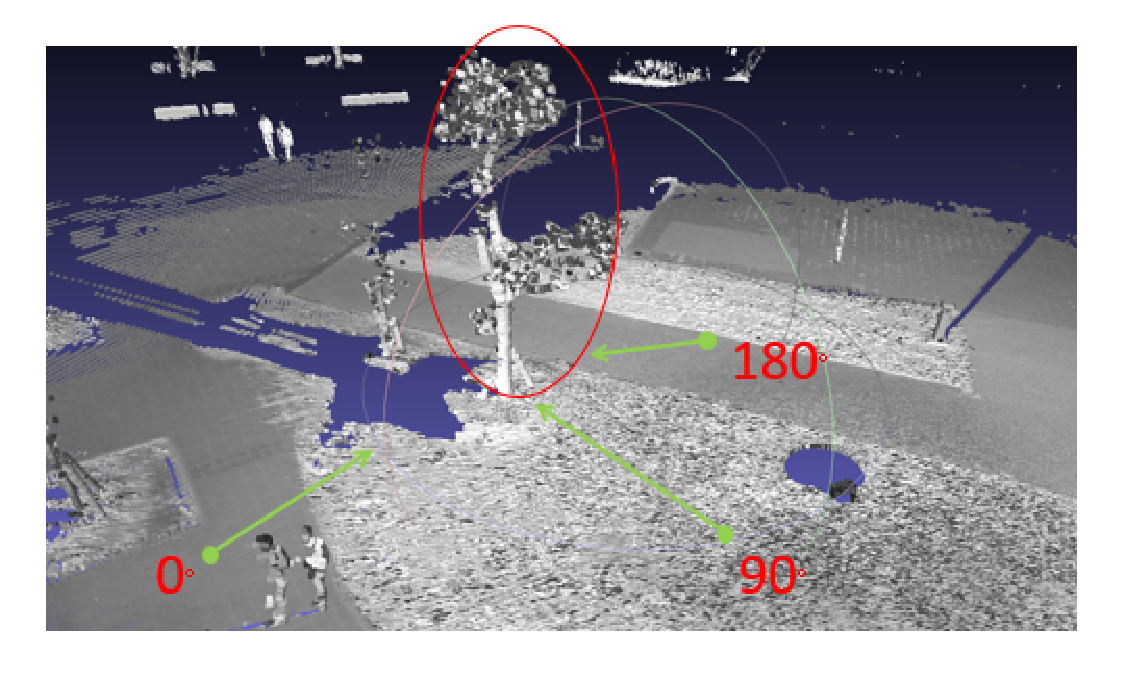
\includegraphics[height=70mm]{figure/一本木の実験場所.eps}
   \caption{一本木の実験場所}
   \label{一本木の実験場所}
  \end{center}
\end{figure}
%

\begin{figure}[htbp]
  \begin{center}
   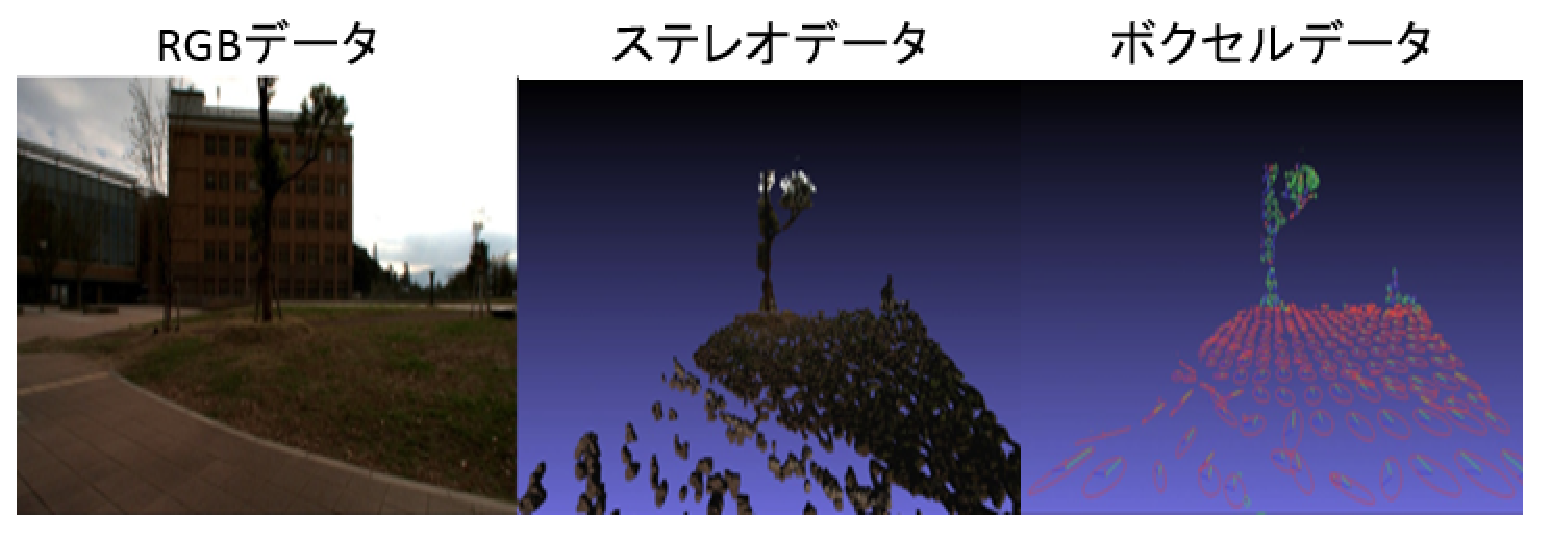
\includegraphics[height=50mm]{figure/0°シーンの各データ.eps}
   \caption{0°シーンの各データ}
   \label{0°シーンの各データ}
  \end{center}
\end{figure}
%
\begin{table}[htbp]
\begin{center}
\begin{tabular}{|c|c|c|c|c|c|} \hline
\  & x(m) & y(m) & z(m) & 距離(m) & 方向(°)\\ \hline
平均誤差 & 0.7 & 0.18 & 0.03 & 0.72 & 1.2\\ \hline
\end{tabular}
\caption{0°シーンの位置同定結果}
\end{center}
\end{table}
%

\begin{figure}[htbp]
  \begin{center}
   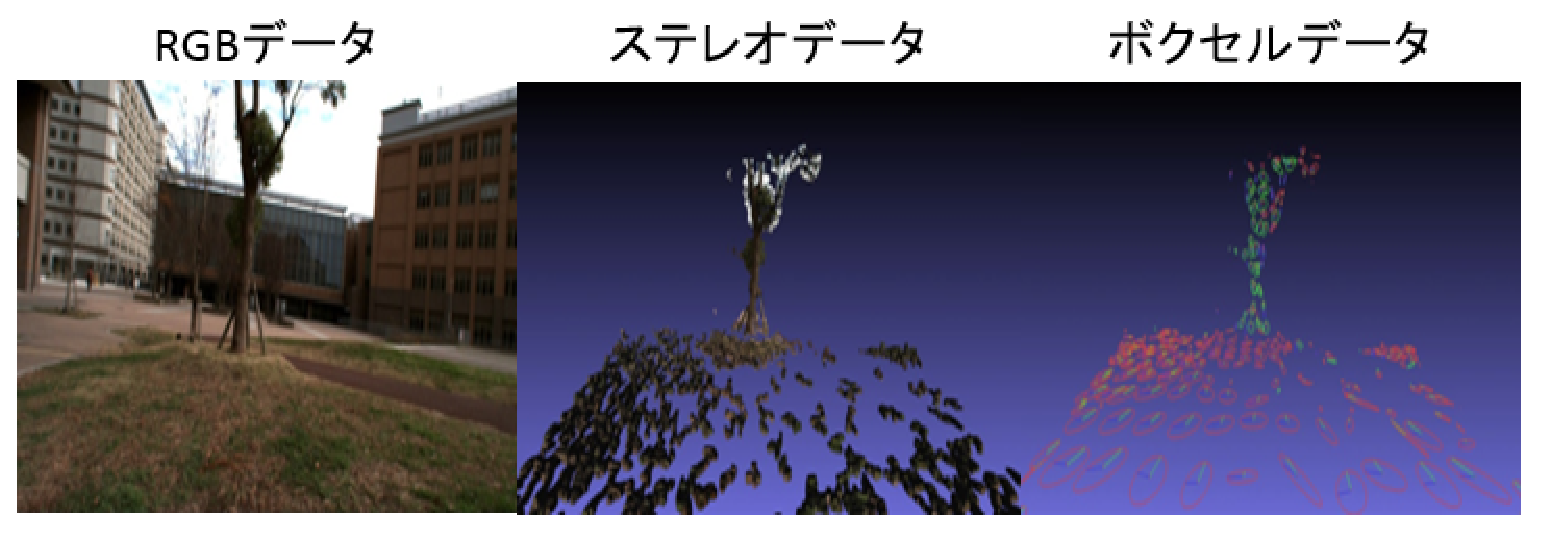
\includegraphics[height=50mm]{figure/90°シーンの各データ.eps}
   \caption{90°シーンの各データ}
   \label{90°シーンの各データ}
  \end{center}
\end{figure}
%
\begin{table}[htbp]
\begin{center}
\begin{tabular}{|c|c|c|c|c|c|} \hline
\  & x(m) & y(m) & z(m) & 距離(m) & 方向(°)\\ \hline
平均誤差 & 0.77 & 2.61 & 0.25 & 2.73 & 146\\ \hline
\end{tabular}
\caption{90°シーンの位置同定結果}
\end{center}
\end{table}
%

\begin{figure}[htbp]
  \begin{center}
   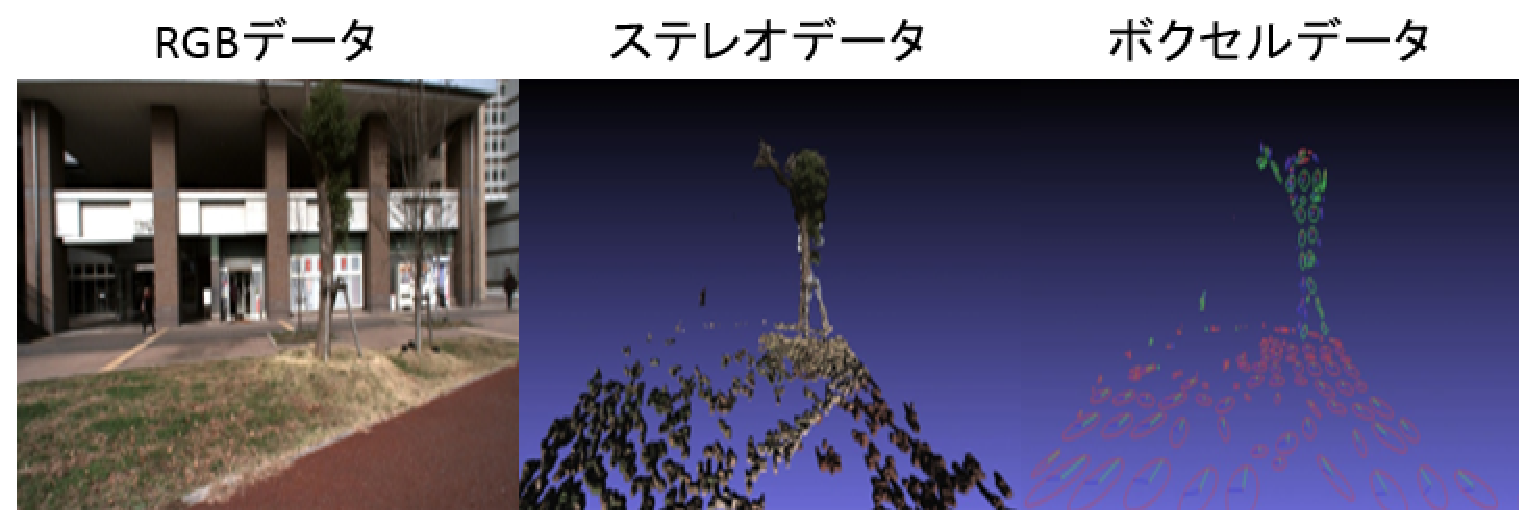
\includegraphics[height=50mm]{figure/180°シーンの各データ.eps}
   \caption{180°シーンの各データ}
   \label{180°シーンの各データ}
  \end{center}
\end{figure}
%
\begin{table}[htbp]
\begin{center}
\begin{tabular}{|c|c|c|c|c|c|} \hline
\  & x(m) & y(m) & z(m) & 距離(m) & 方向(°)\\ \hline
平均誤差 & 0.45 & 0.45 & 0.02 & 0.64 & 7\\ \hline
\end{tabular}
\caption{180°シーンの位置同定結果}
\end{center}
\end{table}
%
\par
図4.28は0°シーンの各データを表し,また,表\hspace{-2mm}4.9に0°シーンの位置同定結果を表す.同じく,図\hspace{-2mm}4.29には90°シーンの各データを表し,表\hspace{-2mm}4.10には90°シーンの位置同定結果を表す.最後に,\hspace{-2mm}180°シーンの各データを図4.30に表し,表4.11に180°シーンの位置同定結果を表す.\par
一本の木の実験は一本だけの木と地面の特徴を用いて位置同定可能有無を確かめる実験であるため,計測データの中で他の木が写っている場合は,木のデータを消す.0°と\hspace{-2mm}180°のシーンを用いた位置同定結果の距離誤差は50cm以上,75cm以下であるが,特徴が一本木と地面しかないことと方向誤差が10°以下であることを踏まえると,ほぼ位置同定ができていると考えられる.しかし,90°のシーンを用いた位置同定では位置同定に失敗している.その理由としては計測データには撮れていないが,地図データを生成するFAROから90°シーンと似ているシーンが撮れているため,位置同定がそこの座標に収束していると思われる.